\documentclass[12pt, letterpaper, titlepage]{report}
% \special{papersize=8.5in,11in}

% Import setup file with includes
\usepackage{authblk}

%%%%%%%%%%%%%%%%%%%%%%%%%%
% ***** Font Setup ***** %
%%%%%%%%%%%%%%%%%%%%%%%%%%
\usepackage{mathptmx}
% \usepackage[T1]{fontenc}

%%%%%%%%%%%%%%%%%%%%%%%%%%%%%%%%%%%%%
% ***** Misc Utility Packages ***** %
%%%%%%%%%%%%%%%%%%%%%%%%%%%%%%%%%%%%%

% TODO Package:
\usepackage{xargs}                      % Use more than one optional parameter in a new commands
\usepackage[pdftex,dvipsnames]{xcolor}
\usepackage[colorinlistoftodos,prependcaption,textsize=tiny]{todonotes}
\newcommandx{\unsure}[2][1=]{\todo[linecolor=red,backgroundcolor=red!25,bordercolor=red,#1]{#2}}
\newcommandx{\change}[2][1=]{\todo[linecolor=blue,backgroundcolor=blue!25,bordercolor=blue,#1]{#2}}
\newcommandx{\info}[2][1=]{\todo[linecolor=OliveGreen,backgroundcolor=OliveGreen!25,bordercolor=OliveGreen,#1]{#2}}
\newcommandx{\improvement}[2][1=]{\todo[linecolor=Plum,backgroundcolor=Plum!25,bordercolor=Plum,#1]{#2}}
\newcommandx{\thiswillnotshow}[2][1=]{\todo[disable,#1]{#2}}

%\usepackage{ifpdf}
% Heiko Oberdiek's ifpdf.sty is very useful if you need conditional
% compilation based on whether the output is pdf or dvi.
% usage:
% \ifpdf
%   % pdf code
% \else
%   % dvi code
% \fi
% The latest version of ifpdf.sty can be obtained from:
% http://www.ctan.org/pkg/ifpdf
% Also, note that IEEEtran.cls V1.7 and later provides a builtin
% \ifCLASSINFOpdf conditional that works the same way.
% When switching from latex to pdflatex and vice-versa, the compiler may
% have to be run twice to clear warning/error messages.

%%%%%%%%%%%%%%%%%%%%%%%%%%%%%%%%%
% ***** Citation Packages ***** %
%%%%%%%%%%%%%%%%%%%%%%%%%%%%%%%%%

\usepackage[
    style=ieee,
    backend=biber,
    sortcites=true,
    sorting=nyt,
%    isbn=false,
   url=true,
   doi=true,
%    eprint=false,
    hyperref=false,
    backref=false,
%    firstinits=false,
    bibencoding=utf8
]{biblatex}

\DefineBibliographyStrings{english}{
    bibliography= {References}
}

\usepackage{csquotes}

%%%%%%%%%%%%%%%%%%%%%%%%%%%%%%%%%
% ***** Graphics Packages ***** %
%%%%%%%%%%%%%%%%%%%%%%%%%%%%%%%%%

\usepackage{graphicx}
\usepackage{hyperref}
% graphicx was written by David Carlisle and Sebastian Rahtz. It is
% required if you want graphics, photos, etc. graphicx.sty is already
% installed on most LaTeX systems. The latest version and documentation
% can be obtained at: 
% http://www.ctan.org/pkg/graphicx
% Another good source of documentation is "Using Imported Graphics in
% LaTeX2e" by Keith Reckdahl which can be found at:
% http://www.ctan.org/pkg/epslatex
%
% latex, and pdflatex in dvi mode, support graphics in encapsulated
% postscript (.eps) format. pdflatex in pdf mode supports graphics
% in .pdf, .jpeg, .png and .mps (metapost) formats. Users should ensure
% that all non-photo figures use a vector format (.eps, .pdf, .mps) and
% not a bitmapped formats (.jpeg, .png). The IEEE frowns on bitmapped formats
% which can result in "jaggedy"/blurry rendering of lines and letters as
% well as large increases in file sizes.
%
% You can find documentation about the pdfTeX application at:
% http://www.tug.org/applications/pdftex

%%%%%%%%%%%%%%%%%%%%%%%%%%%%%
% ***** Math Packages ***** %
%%%%%%%%%%%%%%%%%%%%%%%%%%%%%

\usepackage{amsmath}
\usepackage{amssymb}
\usepackage{amsfonts}
% A popular package from the American Mathematical Society that provides
% many useful and powerful commands for dealing with mathematics.
%
% Note that the amsmath package sets \interdisplaylinepenalty to 10000
% thus preventing page breaks from occurring within multiline equations. Use:
%\interdisplaylinepenalty=2500
% after loading amsmath to restore such page breaks as IEEEtran.cls normally
% does. amsmath.sty is already installed on most LaTeX systems. The latest
% version and documentation can be obtained at:
% http://www.ctan.org/pkg/amsmath

%%%%%%%%%%%%%%%%%%%%%%%%%%%%%%%%%%%%%%%%%
% ***** Specialized List Packages ***** %
%%%%%%%%%%%%%%%%%%%%%%%%%%%%%%%%%%%%%%%%%

\usepackage{algorithmic}
% algorithmic.sty was written by Peter Williams and Rogerio Brito.
% This package provides an algorithmic environment fo describing algorithms.
% You can use the algorithmic environment in-text or within a figure
% environment to provide for a floating algorithm. Do NOT use the algorithm
% floating environment provided by algorithm.sty (by the same authors) or
% algorithm2e.sty (by Christophe Fiorio) as the IEEE does not use dedicated
% algorithm float types and packages that provide these will not provide
% correct IEEE style captions. The latest version and documentation of
% algorithmic.sty can be obtained at:
% http://www.ctan.org/pkg/algorithms
% Also of interest may be the (relatively newer and more customizable)
% algorithmicx.sty package by Szasz Janos:
% http://www.ctan.org/pkg/algorithmicx

%%%%%%%%%%%%%%%%%%%%%%%%%%%%%%%%%%
% ***** Alignment Packages ***** %
%%%%%%%%%%%%%%%%%%%%%%%%%%%%%%%%%%

%\usepackage{array}
% Frank Mittelbach's and David Carlisle's array.sty patches and improves
% the standard LaTeX2e array and tabular environments to provide better
% appearance and additional user controls. As the default LaTeX2e table
% generation code is lacking to the point of almost being broken with
% respect to the quality of the end results, all users are strongly
% advised to use an enhanced (at the very least that provided by array.sty)
% set of table tools. array.sty is already installed on most systems. The
% latest version and documentation can be obtained at:
% http://www.ctan.org/pkg/array


% IEEEtran contains the IEEEeqnarray family of commands that can be used to
% generate multiline equations as well as matrices, tables, etc., of high
% quality.

%%%%%%%%%%%%%%%%%%%%%%%%%%%%%%%%%%
% ***** Subfigure Packages ***** %
%%%%%%%%%%%%%%%%%%%%%%%%%%%%%%%%%%

%\ifCLASSOPTIONcompsoc
%  \usepackage[caption=false,font=normalsize,labelfont=sf,textfont=sf]{subfig}
%\else
%  \usepackage[caption=false,font=footnotesize]{subfig}
%\fi
% subfig.sty, written by Steven Douglas Cochran, is the modern replacement
% for subfigure.sty, the latter of which is no longer maintained and is
% incompatible with some LaTeX packages including fixltx2e. However,
% subfig.sty requires and automatically loads Axel Sommerfeldt's caption.sty
% which will override IEEEtran.cls' handling of captions and this will result
% in non-IEEE style figure/table captions. To prevent this problem, be sure
% and invoke subfig.sty's "caption=false" package option (available since
% subfig.sty version 1.3, 2005/06/28) as this is will preserve IEEEtran.cls
% handling of captions.
% Note that the Computer Society format requires a larger sans serif font
% than the serif footnote size font used in traditional IEEE formatting
% and thus the need to invoke different subfig.sty package options depending
% on whether compsoc mode has been enabled.
%
% The latest version and documentation of subfig.sty can be obtained at:
% http://www.ctan.org/pkg/subfig

%%%%%%%%%%%%%%%%%%%%%%%%%%%%%%
% ***** Float Packages ***** %
%%%%%%%%%%%%%%%%%%%%%%%%%%%%%%
\usepackage{float}
%\usepackage{fixltx2e}
% fixltx2e, the successor to the earlier fix2col.sty, was written by
% Frank Mittelbach and David Carlisle. This package corrects a few problems
% in the LaTeX2e kernel, the most notable of which is that in current
% LaTeX2e releases, the ordering of single and double column floats is not
% guaranteed to be preserved. Thus, an unpatched LaTeX2e can allow a
% single column figure to be placed prior to an earlier double column
% figure.
% Be aware that LaTeX2e kernels dated 2015 and later have fixltx2e.sty's
% corrections already built into the system in which case a warning will
% be issued if an attempt is made to load fixltx2e.sty as it is no longer
% needed.
% The latest version and documentation can be found at:
% http://www.ctan.org/pkg/fixltx2e


%\usepackage{stfloats}
% stfloats.sty was written by Sigitas Tolusis. This package gives LaTeX2e
% the ability to do double column floats at the bottom of the page as well
% as the top. (e.g., "\begin{figure*}[!b]" is not normally possible in
% LaTeX2e). It also provides a command:
%\fnbelowfloat
% to enable the placement of footnotes below bottom floats (the standard
% LaTeX2e kernel puts them above bottom floats). This is an invasive package
% which rewrites many portions of the LaTeX2e float routines. It may not work
% with other packages that modify the LaTeX2e float routines. The latest
% version and documentation can be obtained at:
% http://www.ctan.org/pkg/stfloats
% Do not use the stfloats baselinefloat ability as the IEEE does not allow
% \baselineskip to stretch. Authors submitting work to the IEEE should note
% that the IEEE rarely uses double column equations and that authors should try
% to avoid such use. Do not be tempted to use the cuted.sty or midfloat.sty
% packages (also by Sigitas Tolusis) as the IEEE does not format its papers in
% such ways.
% Do not attempt to use stfloats with fixltx2e as they are incompatible.
% Instead, use Morten Hogholm'a dblfloatfix which combines the features
% of both fixltx2e and stfloats:
%
% \usepackage{dblfloatfix}
% The latest version can be found at:
% http://www.ctan.org/pkg/dblfloatfix




%\ifCLASSOPTIONcaptionsoff
%  \usepackage[nomarkers]{endfloat}
% \let\MYoriglatexcaption\caption
% \renewcommand{\caption}[2][\relax]{\MYoriglatexcaption[#2]{#2}}
%\fi
% endfloat.sty was written by James Darrell McCauley, Jeff Goldberg and 
% Axel Sommerfeldt. This package may be useful when used in conjunction with 
% IEEEtran.cls'  captionsoff option. Some IEEE journals/societies require that
% submissions have lists of figures/tables at the end of the paper and that
% figures/tables without any captions are placed on a page by themselves at
% the end of the document. If needed, the draftcls IEEEtran class option or
% \CLASSINPUTbaselinestretch interface can be used to increase the line
% spacing as well. Be sure and use the nomarkers option of endfloat to
% prevent endfloat from "marking" where the figures would have been placed
% in the text. The two hack lines of code above are a slight modification of
% that suggested by in the endfloat docs (section 8.4.1) to ensure that
% the full captions always appear in the list of figures/tables - even if
% the user used the short optional argument of \caption[]{}.
% IEEE papers do not typically make use of \caption[]'s optional argument,
% so this should not be an issue. A similar trick can be used to disable
% captions of packages such as subfig.sty th\def\BibTeX{{\rm B\kern-.05em{\sc i\kern-.025em b}\kern-.08em
    % T\kern-.1667em\lower.7ex\hbox{E}\kern-.125emX}}
% For subfig.sty:
% \let\MYorigsubfloat\subfloat
% \renewcommand{\subfloat}[2][\relax]{\MYorigsubfloat[]{#2}}
% However, the above trick will not work if both optional arguments of
% the \subfloat command are used. Furthermore, there needs to be a
% description of each subfigure *somewhere* and endfloat does not add
% subfigure captions to its list of figures. Thus, the best approach is to
% avoid the use of subfigure captions (many IEEE journals avoid them anyway)
% and instead reference/explain all the subfigures within the main caption.
% The latest version of endfloat.sty and its documentation can obtained at:
% http://www.ctan.org/pkg/endfloat
%
% The IEEEtran \ifCLASSOPTIONcaptionsoff conditional can also be used
% later in the document, say, to conditionally put the References on a 
% page by themselves.

%%%%%%%%%%%%%%%%%%%%%%%%%%%%%%%%%%%%%%%%%%%%%%%
% ***** PDF, URL AND HYPERLINK PACKAGES ***** %
%%%%%%%%%%%%%%%%%%%%%%%%%%%%%%%%%%%%%%%%%%%%%%%

%\usepackage{url}
% url.sty was written by Donald Arseneau. It provides better support for
% handling and breaking URLs. url.sty is already installed on most LaTeX
% systems. The latest version and documentation can be obtained at:
% http://www.ctan.org/pkg/url
% Basically, \url{my_url_here}.




% *** Do not adjust lengths that control margins, column widths, etc. ***
% *** Do not use packages that alter fonts (such as pslatex).         ***
% There should be no need to do such things with IEEEtran.cls V1.6 and later.
% (Unless specifically asked to do so by the journal or conference you plan
% to submit to, of course. )


% correct bad hyphenation here
\hyphenation{op-tical net-works semi-conduc-tor}

%%%%%%%%%%%%%%%%%%%%%%%%%%%%%%%%%%%
% ---- Paper Specific Setup ----- %
%%%%%%%%%%%%%%%%%%%%%%%%%%%%%%%%%%%
\thispagestyle{plain}   % Makes title page have numbers
\pagestyle{plain}       % Makes other pages have numbers

\bibliography{ref}      % Add bibliography

\doublespacing

\begin{document}

    \title{\textbf{BioMechanical Orthotic Knee Joint for Exoskeletons Thesis} \\
        % {\footnotesize to be used with Microsoft VSCode and Latex}
    }

    \author{\textbf{Alex Tacescu}}

    \affil{
        {Masters Thesis in Robotics Engineering} \\
        {Robotics Engineering Department} \\
        {Worcester Polytechnic Institute}
    }

    \date{May 2021}

    % Make Title Page
    \maketitle

    % Affiliations

    % Make Table of Contents
    \tableofcontents
    \listoffigures
    \listoftables

    \begin{abstract}
    % Short Abstract:
    Current research demonstrates that the shank (lower leg) gets longer as the knee flexes, in a roughly quartic trajectory. However, most actuated orthotics do not consider this tibiofemoral relationship. This thesis presents a customizable biomechanical orthotic knee joint for medical rehabilitation which can follow this relationship. The design is easily manufacturable with common machining tools and FDM 3D printing techniques. Most importantly, it is customizable to each patient with the simple replacement of one component. Finally, this thesis will present a software workflow and tools to identify this tibiofemoral relationship in patients using motion capture technologies.

    % Long Abstract
\end{abstract}



    \chapter{Introduction}
test

    \chapter{Background}

\section{Paraplegia and Rehabilitation}
Paraplegia is a medical term used to define where a patient loses feeling and/or movement in their lower two limbs. In comparison, quadriplegia (also sometimes known as tetraplegia) is the loss of control in all four limbs. It is important to note that not all feeling/movement needs to be lost in order for someone to be considered paraplegic \cite{IncompleteTraumaticQuadrilegia}. Only 30\% of all paraplegic and quadriplegic patients are considered complete lesions, where there is no sensation and no mobility in the lower limbs \cite{RehabParaplegia}. 

\begin{figure} [ht!]
    \centering
    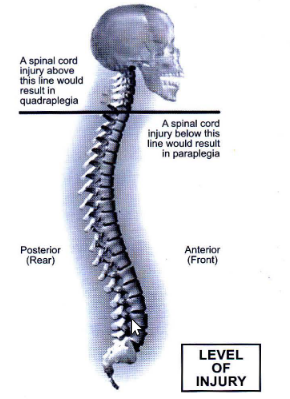
\includegraphics[width=0.5\linewidth]{Figures/Background/ParaQuadInjuryLocs.png}
    \caption{Location of spinal chord injury will determine type of paralysis \cite{RehabParaplegia}}
    \label{fig:ParalysisLocation}
\end{figure}

Paralysis is usually caused by trauma, such as sports injuries, vehicle accidents, or accidental falls, when the spine gets injured (see \autoref{fig:ParalysisLocation}). However, it can also be caused by specific diseases, including multiple sclerosis, amyotrophic lateral sclerosis, stroke, and in specific cases cancer \cite{CausesParaplegia}. Common effects of paraplegia include:
 
\begin{itemize}
    \item Loss of mobility, reflexes, and sensation
    \item Muscular weakness and atrophy
    \item Hormonal variations
    \item Gastrointestinal and bowel/bladder problems
    \item Muscle spasms
    \item Reduced cardiorespiratory fitness and increased likelihood of cardiorespiratory issues
\end{itemize}

Paraplegic and quadriplegic patients also have a higher likelihood of developing skin complications due to their limited mobility and feeling. The limited feeling make skin complications more dangerous, while reduced blood flow to affected limbs increase the recovery time of any dermatological issues \cite{SPISecondaryEffects}. Pressure ulcers are a common example of skin complications in patients suffering from spinal chord injuries, with those suffering from higher levels of paralysis at a higher risk. In fact, a study \cite{PressureUlcerRiskParalysis} discovered that 1/3 of its subjects suffered from at least 1 pressure ulcer in both pre-study analysis as well as throughout the four stages of its study. Therefore, any device to be used with paralysis patients must more-so consider the safety and comfort of the patient.

Rehabilitation can play a key role in reducing these side effects in patients who experience paraplegia. Mainly, physical therapy for paralysis patients focus on three main types of exercises: stretching, strengthening, and aerobic. Additionally, paralysis patients may go through gait training with the assistance of medical devices.

\subsection{Physical Therapy for Paralysis Patients}

\begin{figure}[ht!]
    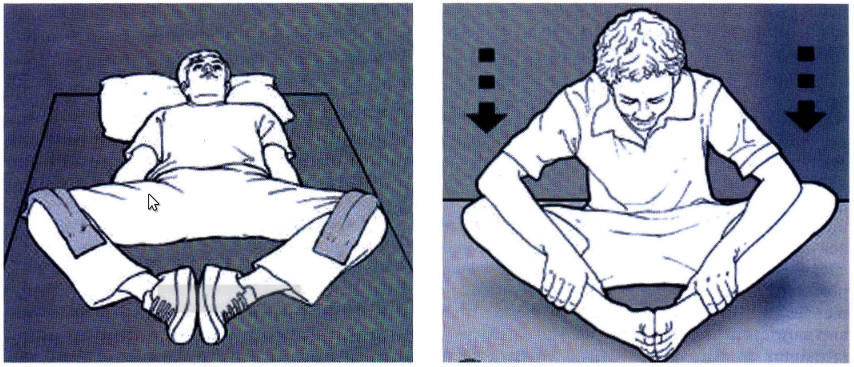
\includegraphics[width=\linewidth]{Figures/Background/BilateralAdductorStretch.png}
    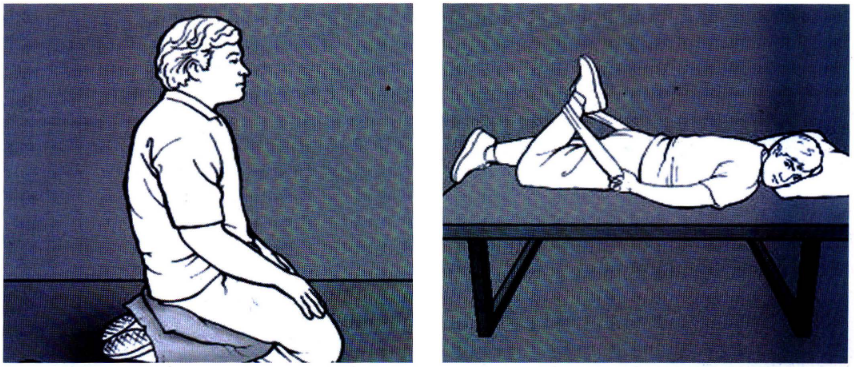
\includegraphics[width=\linewidth]{Figures/Background/QuadricepsStretch.png}
    \caption{Bilateral Adductor Stretches (top) and Quadriceps Stretches (bottom) for paraplegic and quadriplegic patients \cite{RehabParaplegia}}
    \label{fig:ParaplegiaStretches}
\end{figure}

\subsubsection{Stretching}
Stretching is considered one of the most important exercises \cite{RehabParaplegia}, more-so than any other form of exercise because it can be done often and at home. Carefully designed exercises (like seen in \autoref{fig:ParaplegiaStretches}) can improve flexibility, reduce muscle spasms, reduce the chance of injury, and relieve contractures \cite{ParalysisStretchingWeightLoadingPMID} \cite{ParalysisStretchingHarvey} \cite{ParalysisStretchingMichigan}. Some common stretches include bilateral adductor stretches, quadriceps stretches, and hip flexor stretches.

\subsubsection{Cardiorespiratory and Cardiovascular Training}
Due to the difficulty of exercise, cardiovascular and cardiorespiratory activities are also very important to maintain health in paralysis patients. Aerobic exercises can increase energy levels, improve lung and heart function, control body weight, and reduce fatigue \cite{RehabParaplegia} \cite{AerobicCapacityParaplegia}. A study showed that patients who suffer from neuromuscular deficiencies such as paraplegia suffered decreasing VO\textsubscript{2}max \footnote{VO\textsubscript{2}max is a common metric that measures the maximum rate of oxygen utilization during heavy exercise.} compared to control subjects with no issues \cite{AerobicCapacityParaplegia}. The combination of the upper and lower body exercise in paraplegic patients can strengthen the paralyzed limbs while also activating healthy limbs, and ultimately improve the overall health of the patient. Some researchers have even proposed introducing wheelchair racing as a sport in an effort to help with rehabilitation after paraplegia \cite{WheelchairRacingParaplegia}.

\subsubsection{Strength Training}
Improving strength in muscles may actually partially reverse the loss of mobility in partially paralyzed patients, while also improving muscle tone \cite{AerobicCapacityParaplegia} and preventing bone atrophy \cite{ParalysisStretchingWeightLoadingPMID}. This type of exercise can be split into two major regions: training of affected limbs and muscles, and the training of non-affected regions. Affected limbs can benefit from an increase in mobility and definition, and can generally reduce the likelihood of muscular atrophy. Additionally, strong hip and leg muscles in partially paraplegic patients can help in gait training and increase the possibility of usage in life. On the other side, increasing or maintaining strength in unaffected regions can help with quality of life improvement. Often, paraplegic patients may elect to use crutches or canes as an assisted mobility device in the real world. Increasing arm/shoulder strength and endurance will also increase capability for patients to use some of these assisted devices. Finally, back and abdomen muscles are very important to strengthen to maintain posture and improve gait performance \cite{TrunkMuscleLoadingParaplegia}. 

\subsubsection{Hydrotherapy}
Hydrotherapy (exercising in water) is a notable way for patients suffering from paraplegia to better strengthen muscles and improve cardiovascular health. Due to similar buoyancy, water can reduce the effects of gravity without any external assistive devices. At the same time, the increased density of the water (in comparison to air) creates a natural resistance without the use of weights or elastics. Therefore, hydrotherapy is used in paraplegic patients to increase muscle power, increase endurance, and even help with gait training (see \autoref{sec:GaitTraining}). In minor cases of paralysis, some patients even use swimming as a way to exercise \cite{RehabParaplegia} \cite{BenefitsOfHydrotherapy}.

\subsection{Gait Training}
\label{sec:GaitTraining}

Gait training has become the best way to improve motor functions in those who have partially or fully lost mobility in their legs and torso. The premise of this exercise is to have patients do similar movements to what one would do without their disability, like walking and climbing stairs. Essentially, the goal is to help the patient relearn the gaits they previously knew. Spinal neuronal circuits degrade quickly - in just a year, they can lose most of their potency, essentially unlearning any gait abilities the patient had in the past \cite{GaitTrainingClinical} \cite{RehabParaplegia} \cite{TrunkMuscleLoadingParaplegia}. Gait training can help reconnect the broken spinal neurons, and improve motor function and balance in a patient. In fact, several studies have show that some patients with full spinal chord injuries have been able to recover part or even all of their walking capabilities through gait training \cite{GaitTrainingClinical} \cite{ImprovingGaitAdaptabilityInPatients}! 
\footnote{There is significant research in the benefits of gait training for paraplegic and quadriplegic patients. Not all prior work is cited here.} 

\subsubsection{Use of Assistive Devices for Gait Training}
Since most patients suffering from paralysis won't be able to hold themselves up, there have been many different proposals to compensate for gravity. At lower levels of paralysis, canes, walkers, and other walking assisted devices can help. Hydrotherapy has also been used with gait training due to the similar densities of humans and water \cite{BenefitsOfHydrotherapy}. With more serious cases of paralysis, robotic solutions and other active orthotics have been proposed and used in clinical settings.

Standard solutions like canes and walkers will only work for patients with mild paralysis. Canes are designed to support only 25\% of body weight \cite{RehabParaplegia}. They can also be fairly unstable, since they usually only have at most 4 points of contact with a very small ground contact area. Walkers are better than canes, since they can support up to 50\% of body weight \cite{RehabParaplegia}. However, canes, walkers, and crutches have one downside: the required upper-body strength. Mild lower-limb paralysis cases usually can benefit from these inexpensive tools to help with gait training. However most patients will struggle holding themselves up during gait training.

\begin{figure} [ht!]
    \centering
    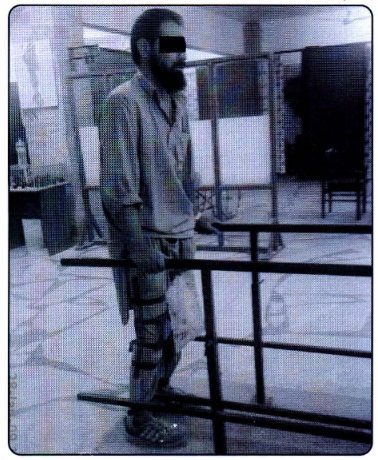
\includegraphics[width=0.4\linewidth]{Figures/Background/SplintsDemo.png}
    \caption{Patient using basic splint orthosis \cite{RehabParaplegia}}
    \label{fig:SplintsDemo}
\end{figure}

Orthosis are the next level up in assistive devices. They can come in many different shapes and can be designed to fit a patient's progress. At the lowest levels are specialty splints or braces (seen in \autoref{fig:SplintsDemo}) that can help keep joints locked or reduce load of a joint through passive springs. These solutions often cost very little in material, and apply normal loads on the user's skeletal system - helping to prevent bone atrophy. Actively powered orthosis also exist with various levels of research and clinical trials (see \autoref{sec:OtherExos}), and can be separated in two major groups. 

\begin{figure}[ht!]
    \centering
    \includegraphics[width=0.4\linewidth]{Figures/Background/OtherExos/LARRE_old.png}
    \hspace*{10mm}
    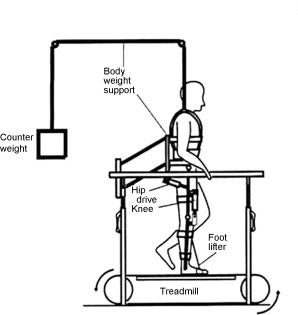
\includegraphics[width=0.4\textwidth]{Figures/Background/ExoSeparateGravityComp.png}
    \caption{Comparison between an exoskeleton with active gravity compensation (left) and an exoskeleton with passive gravity compensation (right) \cite{GaitTrainingClinical}}
    \label{fig:ExoTypesGCSCompared}
\end{figure}

Actively compensating exoskeletons (see left image in \autoref{fig:ExoTypesGCSCompared}) are orthosis devices that use various types of actuators, sensors, and gait controllers to help keep patients standing and walking with little to no strength required (from the patient). These types of exoskeletons use up a significant amount of energy, since they must essentially do all the physical work that leg muscles would normally do. This usually means very powerful actuators and motors with precise and stable control, and large batteries (which add to overall weight) or a large/long tether. Such power increases the overall flexibility of the system, however, at a cost. It also increases complexity of the control software, and introduces a safety risk of attaching powerful actuators to patient limbs.

To mitigate some of these risks, some solutions separate the exoskeleton and the gravity compensation (see right image in \autoref{fig:ExoTypesGCSCompared}). A separate mechanical system supports the weight of the user usually through a counterweight system or a gantry of some sort. This allows for the actuator in the exoskeleton orthosis to be weaker or power (current) limited to prevent injury in case of a malfunction. However, such systems are much more limited in their uses, since the power is hardware limited and more infrastructure is needed to use the device. Additionally, any actively compensating exoskeleton orthosis can be current limited and be used with a mechanical gravity compensation system. 

However, one of the biggest struggles with orthoses is the dermatological problems that they may cause. As explained earlier, patients suffering from paralysis are at an increased risk of developing skin complications \cite{DermatologicalIssuesParalysis}. This can be at least partially attributed to reduced sensitivity in paralyzed areas of the body. Therefore, any assisted devices that attach to a patient's skin should accurately follow the natural trajectory of the skin to avoid unnecessary rubbing.

\subsubsection{Robotics for Paralysis Rehabilitation}
Robotics have a very large opportunity to improve the rehabilitation process in paraplegic patients. Clinical research in using robotic orthosis for gait training and other rehabilitation exercises show positive improvement in most patients when considering quality of life \cite{GaitTrainingBenefitsRoboticsWalkbot} \cite{RoboticGaitTraining}. 
% TODO: [Minor] Add more to this part

\section{Human Knee Model}
\label{sec:KneeModel}

The human knee was initially considered as a pin joint, but research as early as 1992 suggested differently \cite{3DKinKneeJointOldStabby}. This study showed that the joint does extend as it bends by attaching motion capture markers to the femur and tibia of 5 different subjects. It also suggested that there was a difference between loaded and unloaded knees. 
% TODO: [Minor] maybe add more here

\begin{figure}[ht!]
    \centering
    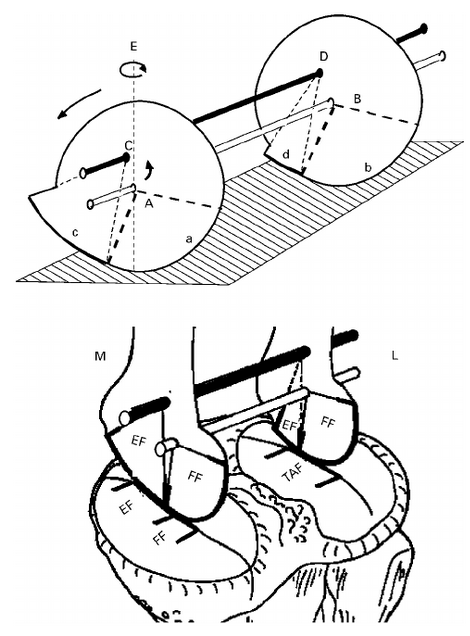
\includegraphics[width=0.5\textwidth]{Figures/Background/KneeAnatomy1.png}
    \caption{Diagram from \cite{MRIKneeShape_Unloaded} depicting the internal anatomy of a knee with respect to the movement patterns. The movement characteristics can be closely related to a cam mechanism}
    \label{fig:KneeAnatomyCam}
\end{figure}

Several studies since then have confirmed a non-linear knee flexion and extension relationship, as well as the difference between loaded and unloaded knees. Instead of intrusive motion capture markers, modern Magnetic Resonance Imaging (MRI) and advanced motion capture systems \cite{ModelAnalysisDeepKneeFlexion} has allowed for more precise bone tracking for both unweighted and weighted knee joints, since a 3 dimensional model can be built of the joint. A study performed by Iwaki \textit{et. al} using MRI data of cadaver knee joints found that the femur posterior circular arc is responsible for the linear extension of the leg through the flexion process, similar to the movement of a mechanical cam (see \autoref{fig:KneeAnatomyCam}) \cite{MRIKneeShape_Unloaded}. Through the bending process, the joint didn't rotate much outside the plane of flexion. These results were further confirmed during the dissection of the cadavers as well as in the followup research with live human knee joints \cite{MRIKneeShape_Loaded}. Additionally, the research also showed tibiofemoral motion moved forward roughly 4mm when the knee joint was loaded.
% TODO: [Minor] Maybe add more here?

\begin{figure}[ht!]
    \centering
    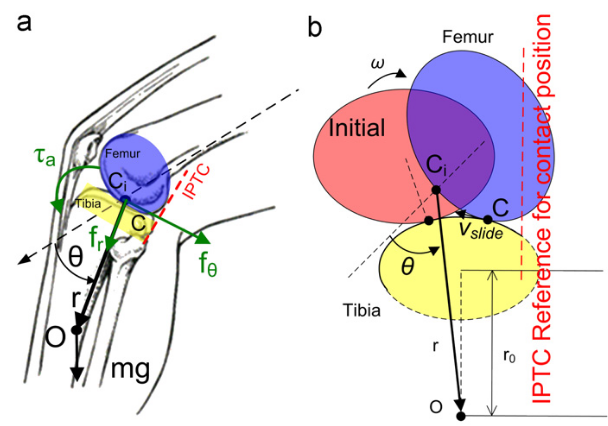
\includegraphics[width=0.8\textwidth]{Figures/Background/KneeParameterization.png}
    \caption{Diagram showing knee rotation \cite{KinDynKneeJoint}: (a) demonstrates the tibia's rotation around an initial contact point \(C_i\). (b) shows the femur and tibia relationship using parameterized shapes between the distance \(r\) and flexion angle \(\theta\)}
    \label{fig:KneeParameterization}
\end{figure}

This research was taken a step further with the parameterization of a knee joint's flexion and extension. The goal was to define a knee joint model to better create artificial mechanisms for rehabilitation exoskeletons. Based on MRI data of unloaded knees from \cite{MRIKneeShape_Unloaded}, ellipses were fitted to the ends of the tibia and femur to approximate the relationship between the distance \(r\) and flexion angle \(\theta\). The resultant tibia to femur relationship can be seen in \autoref{eq:TibiofemoralRelationship} and \autoref{fig:KneeFlexionCurve} \cite{KinDynKneeJoint}.

\begin{equation}
    r(\theta) mm = 1.078\theta^4 - 11.184\theta^3 + 26.524\theta^2 - 0.825\theta + 263.59
    \label{eq:TibiofemoralRelationship}
\end{equation}

\begin{figure}[ht!]
    \centering
    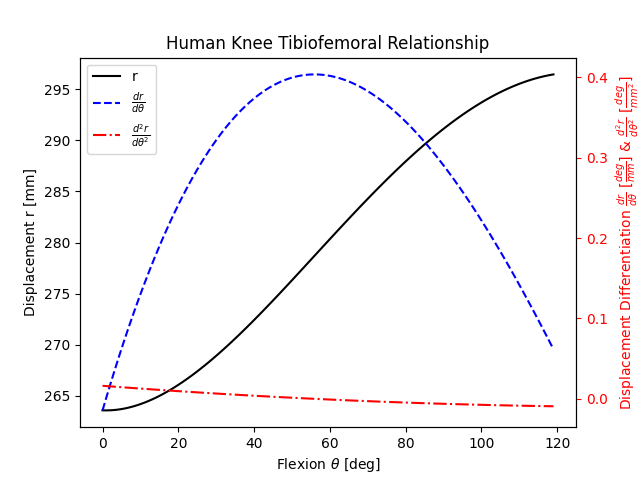
\includegraphics[width=0.9\textwidth]{Figures/Background/FlexionCurve.png}
    \caption{Relationship between tibia and femur during the flexion of the joint. \(r(m)\) is the distance between joint point of contact (\(C_i\) in \autoref{fig:KneeParameterization}) and center of mass of the tibia.}
    \label{fig:KneeFlexionCurve}
\end{figure}

These studies measure the relationship of the bones in the knee joints, and not the skin movement around the joint. However, exoskeleton orthosis are usually connected directly to the skin. In order for the research presented above to be applicable to orthosis, a relationship between the skin and femur/tibia must be made. A study by Benoit \textit{et. al} looked at 8 healthy males to compare the bone and skin movement in and around the knee joint in order to identify if skin markers are sufficient to determine bone kinematics around the knee. Each subject had intra-cortical bone-pins inserted in the proximal tibia and distal femur with 3 motion capture markers on each pin. Then, 8 total motion capture markers were attached directly to the skin to measure the difference in the movement (see \autoref{fig:SkinBoneRelationshipStudy}). 

\begin{figure}[ht!]
    \centering
    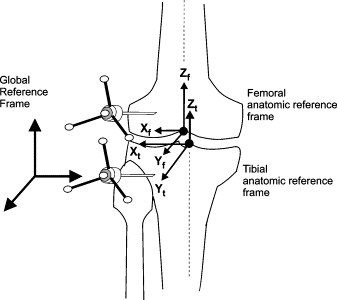
\includegraphics[width=0.6\linewidth]{Figures/Background/SkinMovementResearch_Diagram.jpg}
    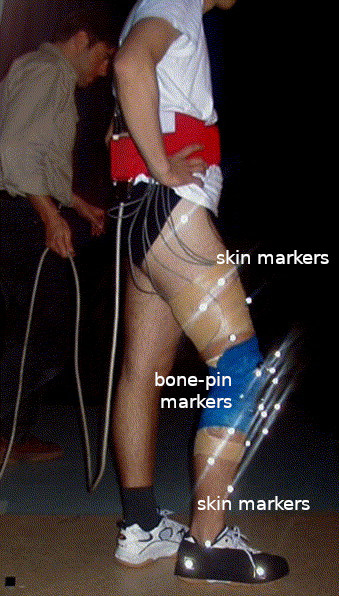
\includegraphics[width=0.3\linewidth]{Figures/Background/SkinMovementResearch_ImageMarked.jpg}
    \caption{Depiction of the research showing the relationship between skin and bone movement: (left) a figure illustrating the location of the bone-pins and (right) showing an image of a subject with all markers attached to them \cite{SkinMovementKneeKin}}
    \label{fig:SkinBoneRelationshipStudy}
\end{figure}

The results of this study seemed to show a significant difference between the skin and bone movement during several different gaits; average rotational errors were between \(4.4^\circ\) and \(13.1^\circ\) while translational errors averaged up to 16.1mm \cite{SkinMovementKneeKin}. What is more interesting is that the errors measured remained relatively constant between different movements, seemingly demonstrating that the error comes from the different connection methods (skin vs bone) and not via measurement tolerances. The researchers were able to conclude that skin-marker kinematics around the knee are not representative of the motion of the bone inside the knee joint. We may be able to therefore inversely conclude that bone kinematics may not be a good representation when designing knee orthoses. However, the research had a relatively small sample size due to the invasive nature of the experiment, and attached markers directly to taped up thighs (see \autoref{fig:SkinBoneRelationshipStudy}), which may have failed to represent the actual skin movement. Therefore, more research is needed to conclude the relationship between a skin connection on the thigh and a skin connection on the shank (calf) for the purpose of rehabilitation exoskeletons.

% Todo: [minor] if time, add a section on knee orthoses
% \subsection{Current Knee Orthoses}


\section{Exoskeleton Orthosis}
\label{sec:OtherExos}
Exoskeletons are an interesting application to help those with paralysis rehabilitate and exercise their muscles. They can take programmatically reduce or add bodyweight to the user to aid with safe gait training and muscle development. Additionally, powered exoskeletons can help move patient legs in the motion of a gait to help with relearning gait cycles such as walking and climbing stairs. The flexibility these rehabilitation devices offer have been noticed, and several different solutions exist at different levels of clinical implementation.

\subsection{WPI LARRE}
\label{sec:larre}
\begin{figure}[ht!]
    \centering
    \includegraphics[width=0.7\linewidth]{Figures/Background/OtherExos/LARRE_old.png}
    \caption{The WPI LARRE rehabilitation exoskeleton \cite{SpringWrapClutchKnee}}
    \label{fig:LARRE_Background}
\end{figure}

The WPI LARRE (Legged Articulated Robotic Rehabilitation Exoskeleton) is an exoskeleton project developed by the \href{http://aimlabdev.wpi.edu} {Worcester Polytechnic Institute (WPI) Automated and Interventional Medicine (AiM) Lab}. The research presented in this thesis directly contributes to the AiM Lab's effort to develop an exoskeleton for rehabilitation of lower-limb paralysis patients. 

The project was originally started and named as the HEX Gen-1. It's goal was to help with studying rehabilitation of patients who have suffered from spinal chord injury using exoskeletons. The project also offers a platform to develop software and hardware technology for rehabilitation exoskeleton. Therefore, it is designed to be adaptable to research different control systems and joint types. The hip joint is powered by a brushless DC motor (Maxon EC90, Maxon Group), while the knee and ankle joints aren't actively powered by any motor. Instead, the knee joint contains a spring wrap clutch/brake to help provide support to patients throughout their gait cycles as proposed by \cite{SpringWrapClutchKnee}. Additionally, the ankle joint included a spring to add force during dorsiflexion to help in walking gaits.

\subsection{H2}

\begin{figure}[H]
    \centering
    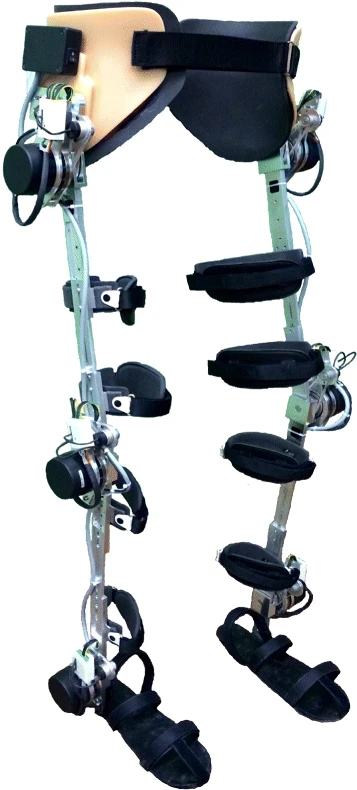
\includegraphics[width=0.3\linewidth]{Figures/Background/OtherExos/H2_Exo.png}
    \hspace{0.1\linewidth}
    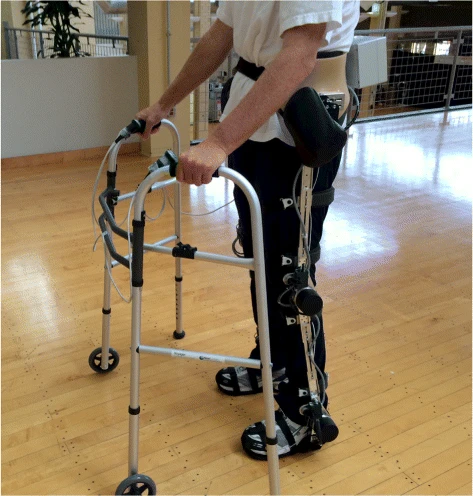
\includegraphics[width=0.5\linewidth]{Figures/Background/OtherExos/H2_ExoUse.png}
    \caption{The H2 Exoskeleton, with 6 powered joints and lithium polymer batteries \cite{ExoH2}}
    \label{fig:H2Exo}
\end{figure}

The H2 robotic exoskeleton is designed by the University of Houston to help stroke survivors with gait training and physical rehabilitation. It has 6 powerful DC motors (3 on each leg on the hip, knee, and ankle joint) geared down with harmonic gearboxes. Each motor is powered by its own local motor controller, with all electronics connected to a main controller via CAN bus. An assistive gait controller is used to apply torque when patients deviate from a planned gait pattern. The device itself was tested on 3 hemiparetic stroke patients, and was safe and effective throughout the 4 week testing period. The pilot clinical study demonstrated the "assist-as-needed" control system was able to benefit the stroke patients, and help them recover \cite{ExoH2}.

\subsection{ReWalk}
\begin{figure}[H]
    \centering
    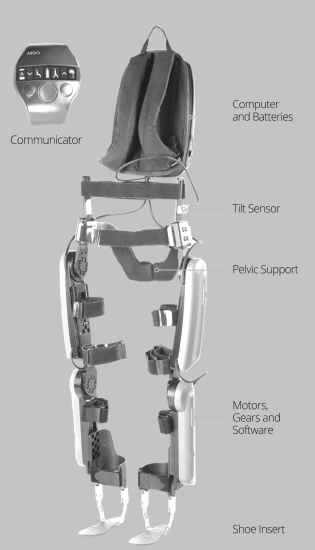
\includegraphics[width=0.4\linewidth]{Figures/Background/OtherExos/ReWalk.png}
    \caption{The Rewalk exoskeleton: an commercial exoskeleton with knee and hip powered joints \cite{ExoRewalk}.}
    \label{fig:RewalkExo}
\end{figure}

The {Rewalk\texttrademark} exoskeleton (Rewalk Robotics) is a commercial exoskeleton for lower-limb paralysis patients. Unlike most medical exoskeletons, Rewalk is designed for daily use - not just for rehabilitation in controlled environment. It consists of a lower-limb exoskeleton with powered rotary joints. The joints do not consider tibiofemoral joint trajectory, and have a static center of rotation. The system is all powered by a computer and batteries in a backpack worn by the user. Research by Talaty \textit{et. al} in \cite{ExoRewalk} demonstrated that assistive devices such as Rewalk are able to improve the walking capability of lower-limb paralysis patients with some practice. 

\subsection{EksoNR}
\begin{figure}[H]
    \centering
    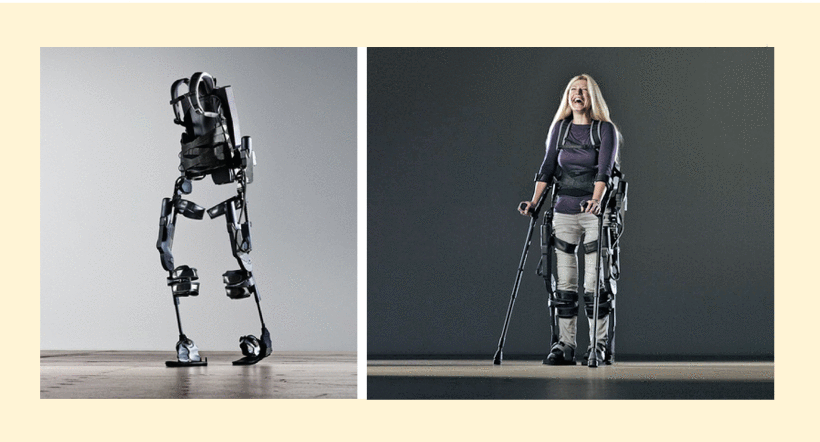
\includegraphics[width=0.9\linewidth]{Figures/Background/OtherExos/EKSO.png}
    \caption{The Ekso exoskeleton is a commercial rehabilitation system currently used in hospitals and rehabilitation centers.}
    \label{fig:EksoExo}
\end{figure}

The EksoNR exoskeleton (EksoBionics, Richmond California) is a commercial rehabilitation exoskeleton currently in clinical use since February 2012. EksoBionics - the company that manufactures this device - claims to be the only FDA-cleared exoskeleton for use with patients with acquired brain injury which has lead to paralysis. It has similar functionality and features to the Rewalk; the hip, knee, and ankle joints are all actuated pin joints. The exoskeleton holds the control electronics and batteries in a backpack-like container, which doubles as a way to stabilize the patient's upper body during use \cite{ExoEksoNR}.

% \subsection{Indigo}

% \subsection{KINESIS}

% \subsection{HAL}

    \chapter{Knee Joint Design}

The knee joint presented in this thesis is designed to replace the current passive pin knee joint with a spring wrap clutch for the WPI LARRE exoskeleton (see \autoref{sec:larre}).

\TODO{add more in the intro section for the knee joint design}

\section{Design Parameters}

\subsubsection{Follow a specific equation}

\begin{equation}
    r(\theta) mm = 1.078\theta^4 - 11.184\theta^3 + 26.524\theta^2 - 0.825\theta + 263.59
    \label{eq:KneeJointGeometryEquation}
\end{equation}

\subsubsection{Parameter 2}


\section{Mechanical Design}

The orthotic joint design proposed uses a similar idea to how a human knee joint works; a cam mechanism  extends the shank link as it is rotated relative to the thigh link. The joint therefore has two degrees of freedom: rotation around the center of rotation (output shaft of the motor and gearbox) and translation in the direction of the shank. However, since there is only one actuator, the joint is underactuated; this underactuation can be taken advantage of to match a patient's knee trajectory, where the center of mass of the shank extends away from the joint center as the joint bends.

\begin{figure} [ht!]
    \centering
    \missingfigure{Knee Joint Exploded View}
    \caption{Exploded view of the knee joint, with all relevant components labeled}
    \label{fig:KneeJointExplodedView}
\end{figure}

\subsubsection{Torsion Bars}
The center of rotation of the joint is designed to match the axis of rotation of the actuator. The output of this actuator \fix{Add reference to actuator decision section} is directly connected to the torsion bar using M5 shoulder bolts. Each bolt is designed to support 3 bearings: 2 on the motor side and 1 on the patient side. The reduced count on the patient side allows for the torsion bar to be partially recessed in the shank link to reduce the distance between the center of mass between the patient and the joint. The 6 bearings are still able to support the forces necessary throughout a walking gait cycle (see \autoref{sec:BearingsAndCalcs}). 

\subsubsection{Shank Links}
The 2 shank links attach to the lower part of the exoskeleton, and are responsible for taking the rotational energy created by the motor and partially changing it to translational energy to help linearly extend the shank. The bearings connected to the torsion bars ride in a guide built into the shank link. This guide is slightly larger than the bearing diameter (\(~0.3mm\)) to prevent rubbing without creating much of a backlash (\(0.39^\circ\) backlash, see calculation on \autoref{eq:ShankLinkBacklash}).

\begin{equation}
    Backlash = atan(\frac{\frac{0.3mm}{2}}{22mm}) = 0.39^\circ
    \label{eq:ShankLinkBacklash}
\end{equation}

The surface of the guide must be smooth and parallel to the axis of the bearings to avoid damaging them. Depending on the material and manufacturing method chosen, the surface may require additional machining to ensure it can match these requirements. The length of the guide must be larger than the distance between the centers of the two shoulder bolts plus the maximum distance of linear extension by the knee (\autoref{eq:ExtensionGuideLength}). For this prototype, this length was \(78mm\).

\begin{equation}
    GuideLength \geq TorsionBarC2C + MaxKneeExtension = 44mm + 34mm = 78mm
    \label{eq:ExtensionGuideLength}
\end{equation}

The shank link is also responsible to connect to the lower part of the exoskeleton. Just like the thigh link, this is done through the universal exoskeleton connector developed throughout the WPI LARRE project \cite{SpringWrapClutchKnee}.

The connection between the thigh link and the shank link is very important, as it adds torsional stability and overall rigidness to the entire joint. It was therefore imperative during the design process to create wide surface contact between the thigh and shank links. To reduce the energy lost to friction between these plates, 3.2mm thick Delrin\textsuperscript{\textregistered} slides were laser cut and attached to the shank link. 

Similarly to the torsion bar, the shank link also uses 2 shoulder bolts to clamp the two shank links on the thigh link as well as to give the bearings that ride on the knee path guide a precise surface to mount to. To maintain a consistent clamping force, lock nuts are used since they do not easily back out with movement and vibration. 

\subsubsection{Thigh Link}

\begin{figure}
    \centering
    \missingfigure[]{Add cross section of the joint}
    \caption{A cross section of the knee joint in a \(0^\circ\) position}
    \label{fig:KneeJointCrossSection}
\end{figure}

The thigh link acts as the main mounting point for most things, as well as contains the knee path guide. Just like the shank link, the thigh link has the universal exoskeleton connector used throughout the WPI LARRE project. The motor bracket is connected to the thigh link at two locations using \(20mm\diameter x 50mm\) spacers. These spacers must be strong and stiff, as they transmit the torque between the thigh and shank connector in high load situations. A potentiometer is also mounted inside the thigh link to measure the current angle of the joint, as shown in \autoref{fig:KneeJointCrossSection}. The wire connecting to it is routed through a slot in the thigh link to avoid any interference with the moving shank links. This wire comes out the top and is connected to the main controller of the exoskeleton.

\subsubsection{Knee Path Guide}
The knee path guide is built into the thigh link as a slot. The geometry is calculated using several point measurements connected in SolidWorks with a spline. Each point is split by \TODO{Verify this number}{15 degrees}, and calculated from a pre-determined equation. This equation can be measured from a patient knee (see \autoref{sec:KneeParams}), but throughout the design and testing of this knee joint, \autoref{eq:KneeJointGeometryEquation} from \cite{KinDynKneeJoint} is used. \autoref{fig:CenterPlateGeometry} shows the equation above overlayed on the thigh link.

\begin{figure}[ht!]
    \centering
    \missingfigure{Make a picture of the thigh link with relationship highlighted}
    \caption{The thigh link contains the geometry which the bearings ride on to mimic the tibiofemoral relationship}
    \label{fig:CenterPlateGeometry}
\end{figure}

The joint is designed to be easily adaptable between patients. Therefore, the only customized part in the entire system is the thigh link which holds the knee path guide. All other parts remain the same to decrease cost and improve repairability.

\subsubsection{Torque Requirements \& Actuator Selection}

\begin{figure}[ht!]
    \centering
    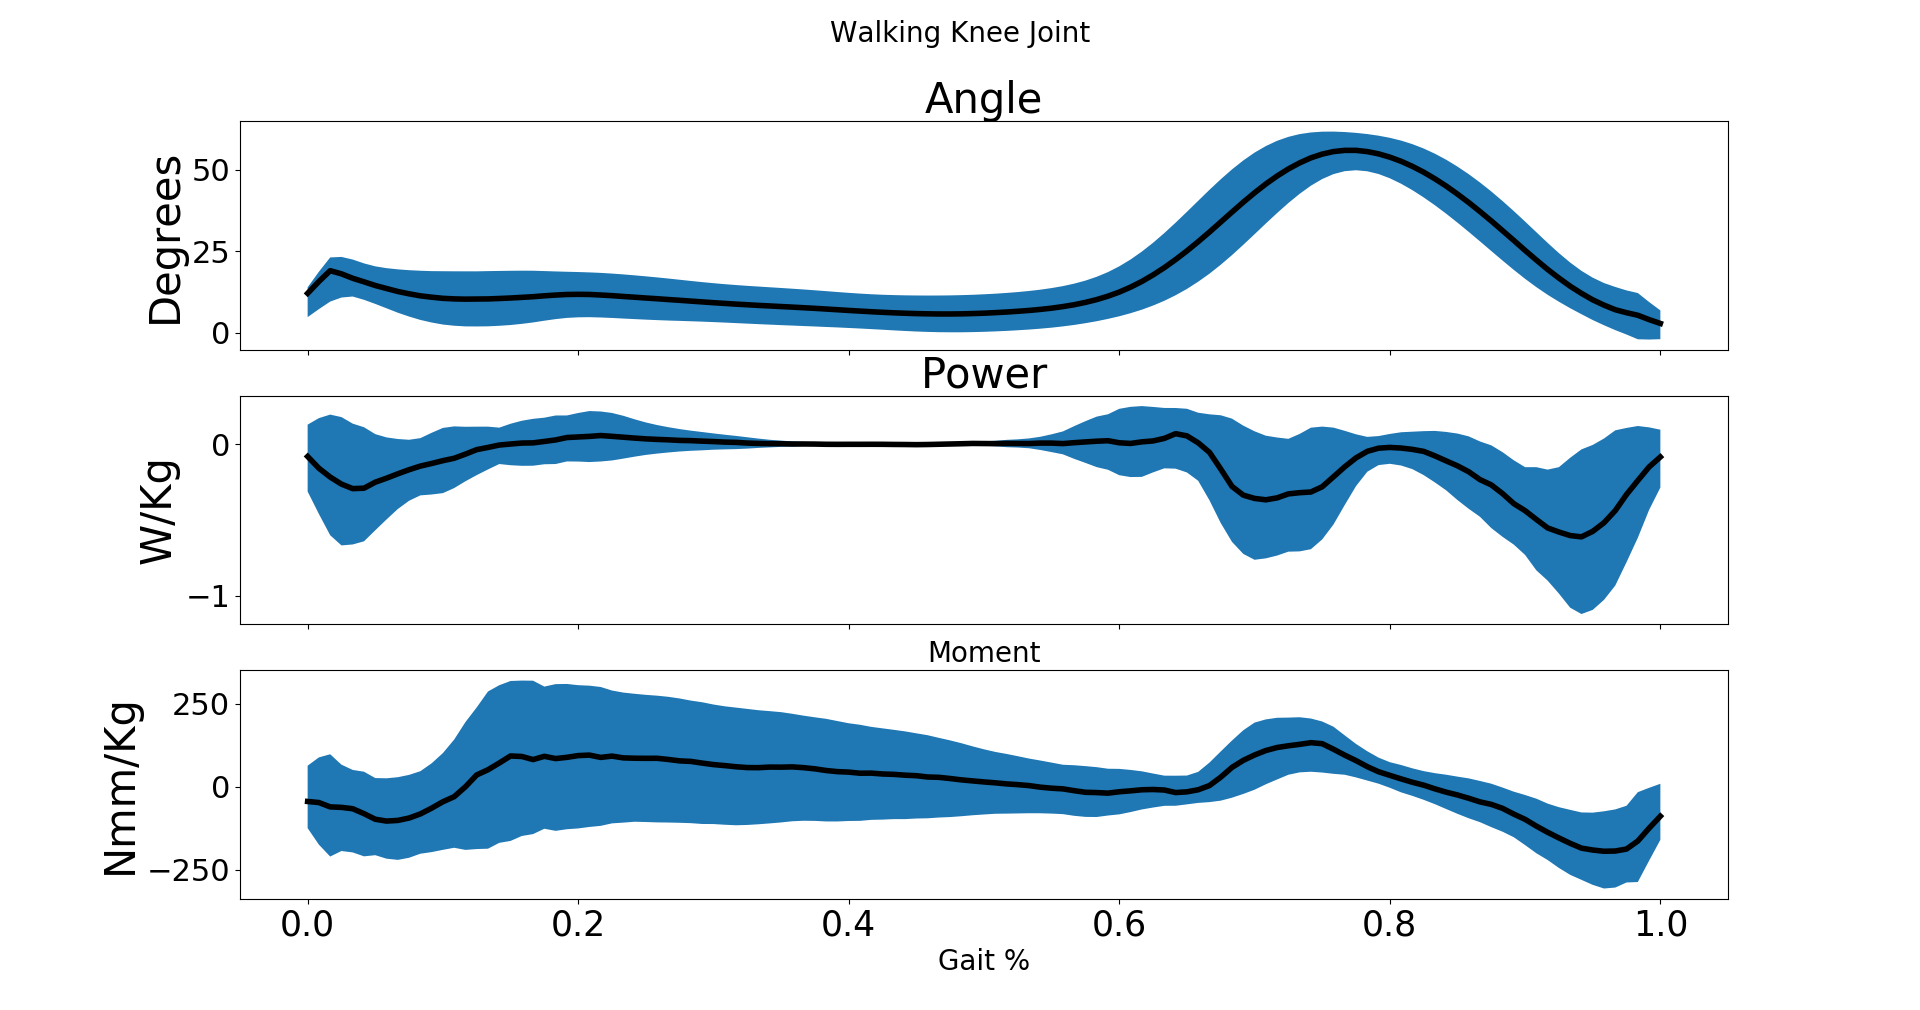
\includegraphics[width=\linewidth]{Figures/Design/WalkingPowerCurveKnee.png}
    \caption{Joint kinematics and dynamics during a walking gait cycle \cite{SpringWrapClutchKnee}}
    \label{fig:WalkingPowerCurve}
\end{figure}

\begin{figure}[ht!]
    \centering
    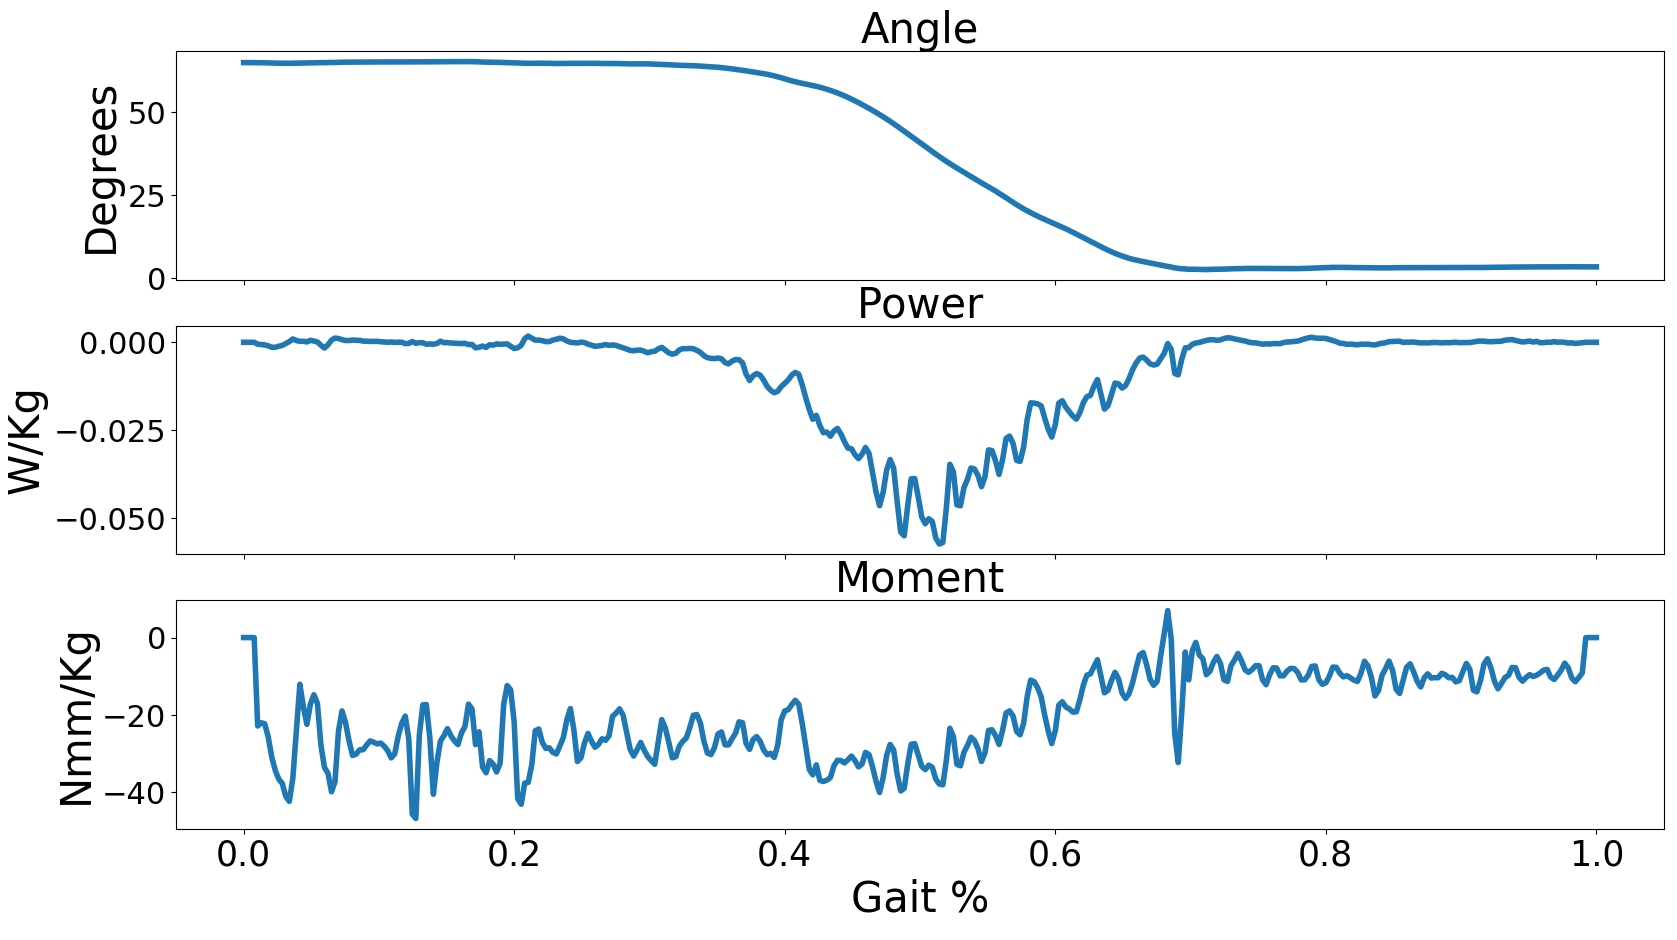
\includegraphics[width=\linewidth]{Figures/Design/SitStandPowerCurveKnee.png}
    \caption{Joint kinematics and dynamics during a sit/stand gait cycle \cite{SpringWrapClutchKnee}}
    \label{fig:SitStandPowerCurve}
\end{figure}

The knee joint has two rehabilitation requirements to fulfill: walking gaits and sit/stand gaits. Prior research has shown that walking gaits require roughly up to \(0.65 \frac{W}{kg}\) and \(0.25\frac{Nm}{kg}\), (see \autoref{fig:WalkingPowerCurve}), while a sit/stand gait requires roughly up to \(0.5 \frac{W}{kg}\) and \(0.04 \frac{Nm}{kg}\). Therefore, the chosen maximum parameters for this knee joint with a \(100 kg\) weight specification is \(65 W\) and \(25 Nm\). \footnote{Peak power reported by the motion capture data is higher, but these parameters were chosen after noise is filtered out. The data is recorded from a normal walking gait of a healthy person.} Speed requirements are roughly \(12^\circ/sec\) for walking gaits and \(15^\circ/sec\) for sit/stand gaits.

The Maxon EC90 was chosen, with a peak power output of \(90W\) and a max continuous torque of \(0.560 Nm\) at \(2510 rpm\) (see \autoref{apx:EC90Datasheet}). To match the speed and torque requirements, a \(100:1\) gearbox ratio is needed. Due to its high reduction to size ratio, a strain wave gearbox from {Harmonic Drives\texttrademark} was chosen.\footnote{The gearbox used is proprietary, and no datasheet is available} Estimated efficiency of this gearbox is roughly \(\epsilon = 90\%\).

\begin{table}
    \centering
    \begin{tabular}{||c|c|c||}
        \hline
        Input (Motor) Power & \(P_{input}\) & \(90 Watts\) \\
        \hline
        Input (Motor) Torque @ Nominal & \(\tau_{input}\) & \(0.560 Nm\) \\
        \hline
        Input (Motor) Speed @ Nominal & \(\omega_{input}\) & \(2510 rpm\) \\
        \hline
        Input (Motor) Stall Torque & \(\tau_{in\_stall}\) & \(7.480 Nm\) \\
        \hline \hline
        Gearbox Ration & \(\frac{n_1}{n_2}\) & \(100:1\) \\
        \hline \hline
        Output Power & \(P_{output}\) & \(81 Watts\) \\
        \hline
        Output Torque @ Nominal & \(\tau_{input}\) & \(50.4 Nm\) \\
        \hline
        Output Speed @ Nominal & \(\omega_{input}\) & \(15^\circ/sec\) \\
        \hline
        Output Stall Torque & \(\tau_{out\_stall}\) & \(673.2 Nm\) \\
        \hline
    \end{tabular}
    \caption{Motor/gearbox specifications and output power specifications of the proposed joint. See \autoref{apx:JointPowerTorqueSpeedCalcs} for all equations and calculations used.}
    \label{table:MotorGearboxSpecs}
\end{table}

The output power of the joint is \(81 W\), with a nominal torque of \(50.4 Nm\) at \(15^\circ/sec\). Power, torque, and speed specifications of the joint theoretically exceed the requirements. Physical testing is needed, however, to ensure that these numbers are accurate and sufficient for a rehabilitation exoskeleton.
 
\subsubsection{Potentiometer and Rotary Encoder}
A potentiometer was embedded into the knee design to act as an absolute rotary encoder to measure the current angle of the joint. It's purpose is twofold: to provide for an absolute angle at any given time and to provide for rough rotary encoding when a the motor (for passive experimentation). As mentioned above, the integration needed to protect the sensitive connection points. The potentiometer chosen was the Vishay PRV6, with \(200^\circ\) of travel, a linear resistance, and \(\pm 1\%\) tolerance, which equates to a sensored tolerance of \(\pm 2^\circ\). 

The motor used also has 3 hall sensors used for pinpointing the position of the rotor versus the stator. Since the motor has a 12 poles and 3 sensors (totaling 36 pulses per revolution) as well as a 100:1 reduction through the gearbox, the hall effect sensors can be used to create an effective 3600 pulses per revolution encoder. When used in conjunction with the absolute encoder, the encoded angle can be very precise.

% \subsubsection{Motor Analog} 
% \TODO{change the name of this}
% \TODO[inline]{Talk about motor/gearbox analog}

\section{Manufacturing, Materials, \& Parts}
Throughout the design, manufacturability and easy assembly was a focus. The entire system is held together with 4 M5 shoulder bots with 6mm diameter shoulders to be used as an accurate bearing surface.

\subsubsection{Bearings}
\label{sec:BearingsAndCalcs}
All 10 bearings used in the design are the same (for simplicity and reduction of cost): 19mm outside diameter x 6mm inside diameter x 6mm thick double shielded ball bearings (Model 626ZZ). Each is rated for \(2.6kN\) dynamic load and \(1.05kN\) static load. Before selecting these bearings, two calculations were required to ensure these bearings could support the forces required.

The first is the requirement of the torsion bar. 

The second force requirement for these bearings were in the knee path cam

\section{Testing \& Results}

\subsection{Material Analysis}

\subsection{Simulation Motion Analysis}

\subsection{Real-world Motion Analysis}


    \chapter{Parameterization of Human Knee Joints}
\label{sec:KneeParams}

The proposed and prototyped knee joint requires a specific input of patient parameters to achieve its goal of matching a person's knee movement. Therefore, a system must be developed to non-invasively identify a relationship between the flexion of the patient's knee joint and the linear movement of the shank away from the knee's joint center. There have been several attempts to parameterize the human knee joint using many different methods, including \cite{3DKinKneeJointOldStabby}, \cite{MRIKneeShape_Unloaded}, \cite{MRIKneeShape_Loaded}, and \cite{ModelAnalysisDeepKneeFlexion}. All of these studies focus on the tibiofemoral relationship, i.e. the bone movement within the lower limbs. However, rehabilitation exoskeletons connect to the skin of its user. Other studies have identified a difference between identifying knee kinematics through skin markers and bone pins \cite{reinschmidt1997effect}, suggesting there is in fact a distinct difference between tibiofemoral movement and skin movement around the knee. Therefore, an imaging workflow and software processing program needs to be developed to be able to parameterize a patient's knee movement with consideration to skin movement.

To identify the knee relationship, an imaging workflow as well as an accompanying software analysis tool is proposed and tested with pilot data. This imaging method uses a motion capture system to identify movement of specific markers attached to a person's skin. This will all be processed using a custom software workflow consisting of both Vicon image processing and custom Python scripts that will extract the parameters from the data. To test this workflow, an experiment is proposed using medical MR imaging to identify the kinematics of the knee joint, compare the developed knee joint to a traditional pin joint, and determine the relationship between the knee joint kinematics and the skin movement surrounding the knee.

\section{Proposed Method of Imaging}
\label{sec:ImaginKneeProcedure}

\begin{figure}[ht!]
    \centering
    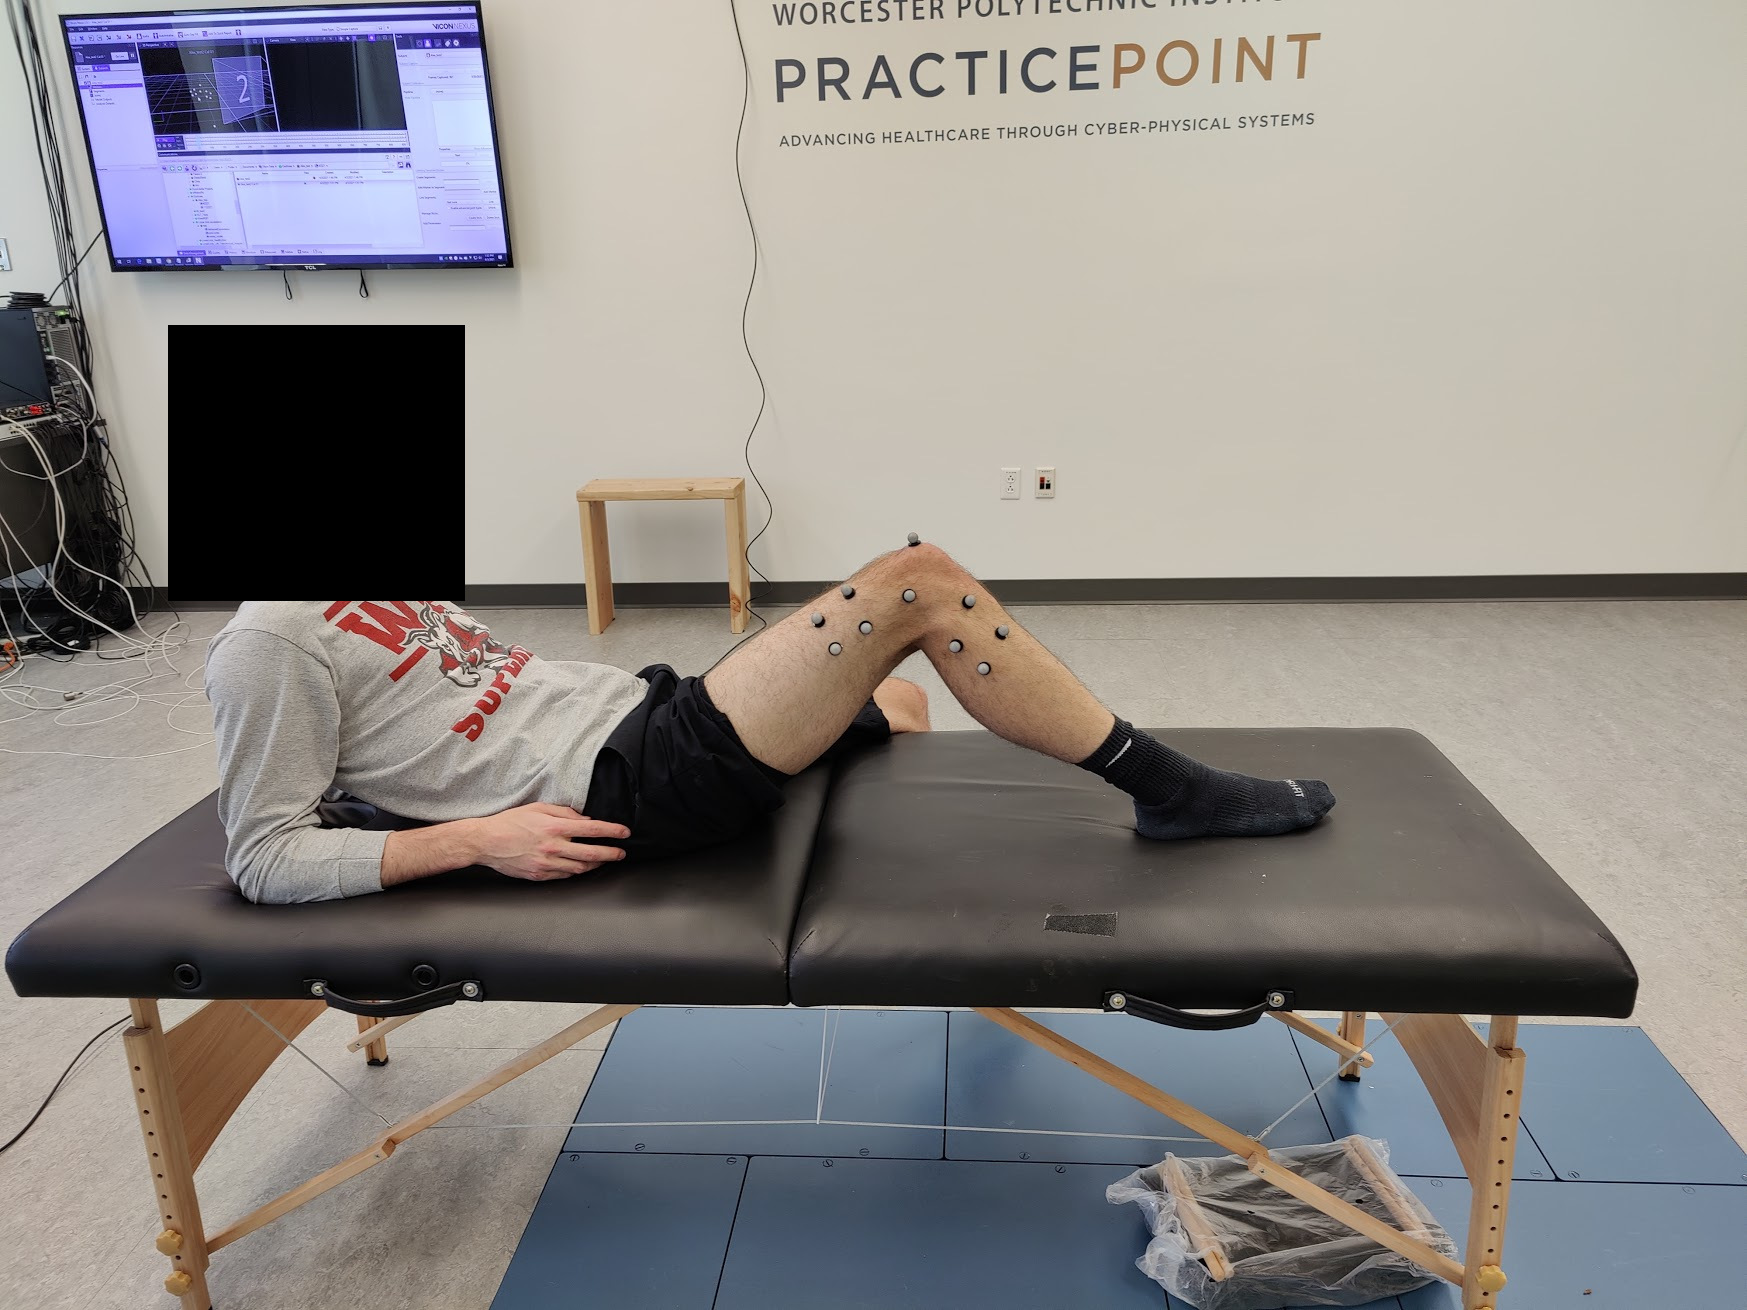
\includegraphics[width=0.65\textwidth]{Figures/Param/StudyPatientPositioning.jpg}
    \caption{Depicts the patient position during motion capture. The patient will then flex and extend their knee while keeping the heel on the table.}
    \label{fig:ParamPatientPosition}
\end{figure}

The proposed imaging workflow can be split up into two major parts: the imaging session and the software processing. For flexibility and speed, the usage of a motion capture system is proposed, which can develop accurately track the position of motion dots. In this study, the motion capture system used was a 10-camera Vicon Vantage 5 \footnote{See Vicon system here: \url{https://www.vicon.com/hardware/cameras/vantage/}}, but any motion capture system is usable given enough precision. 

To measure the knee flexion, a patient is placed on their back, shown in \autoref{fig:ParamPatientPosition}.Motion capture dots are then placed on the patient using double-sided tape to track the positions where the exoskeleton will attach to the skin. Two additional points can be placed on the knee for extra feedback and the final joint position, but are not necessary for the software system. Then, the patient will flex and extend their knee joint while keeping the heel on the table to stabilize the knee and prevent shanking. The placement of the patient should allow for a technician to help the patient bend their knee if their condition does not allow them to do so themselves. Once the data is collected, it can be processed by the parameterization software system.

\section{Parameterization Software}
% TODO: Add software flowchart
The collected data first goes through a Vicon workflow for processing. This will properly format the data, create virtual joints, and determine joint centers. This is done using the built-in tools called SCoRE (Symmetrical Center of Rotation Estimation) and SARA (Symmetrical Axis of Rotation Analysis). Additionally, a built-in tool will determine the angle of the knee joint using the four dots on each section of the patient's leg. This Vicon specific workflow can be exported, shared, and reused for others who are using a similar system. The output of the workflow is a CSV file which can be parsed by a custom script.

To finish the parameterization of the knee, custom software was developed and written in Python. This software utilizes the AiM Vicon Python module \footnote{The AiM Vicon Python module is an open-source project found here: \url{https://github.com/WPI-AIM/AIM_Vicon}} which parses the CSV file from above. The joint angle, SARA, SCoRE, and marker positions are extracted from the data and placed in their specified datatypes. Since the AiM Vicon module did not have all the tools needed for this project, I developed and contributed to the Python module. Additional features added include SARA and SCoRE support, a new 3D visualizer, and stability improvements when importing different workflows.

\begin{figure}[ht!]
    \centering
    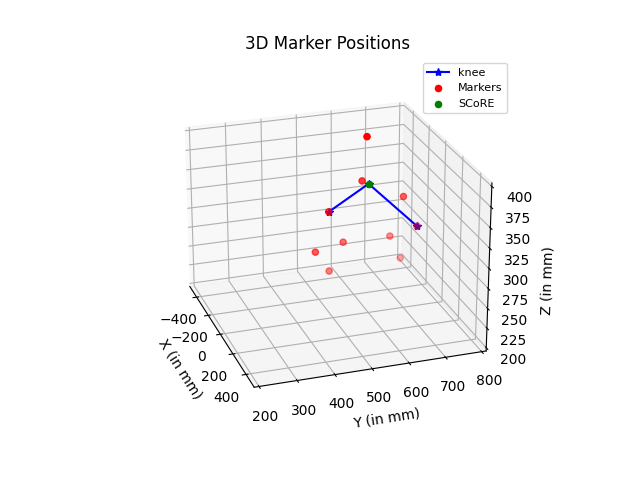
\includegraphics[width=\textwidth]{Figures/Param/3D_Marker_Animation.png}
    \caption{An example of a possible output from the Parameterization Software System shown in a visualizer}
    \label{fig:SoftwareSampleData}
\end{figure}

With the data parsed and imported, the final step is to calculate the final joint angles and determine the linear extension between the thigh and shank. The axis of rotation from SCoRE and all marker positions are projected onto a plane, which is calculated to be approximately the same as the plane of the manufactured joint. Then the final distance and angle are calculated by drawing two virtual lines as shown in \autoref{fig:SoftwareSampleData}: 1. from the projected primary thigh marker to the projected SCoRE location and 2. from the projected SCoRE location to the projected primary shank marker. The lengths of these lines then become the calculated linear extension and the angle between these two lines become the flexion. These two metrics are then combined into a dataset, and a best fit quartic curve is selected to become the patient's knee parameters.

\section{Testing with Pilot Data}
Due to time constraints, IRB (Internal Review Board) approval was not obtained to run a full study. However, some data was used to develop the software platform that will analyze the data. The graphs in \autoref{fig:Subj1KneeParams} and \autoref{fig:Subj2KneeParams} show the relationships between the knee joint flexion (angle of the knee) and the linear extension (distance of the shank to the joint center).

\begin{figure}[ht!]
    \centering
    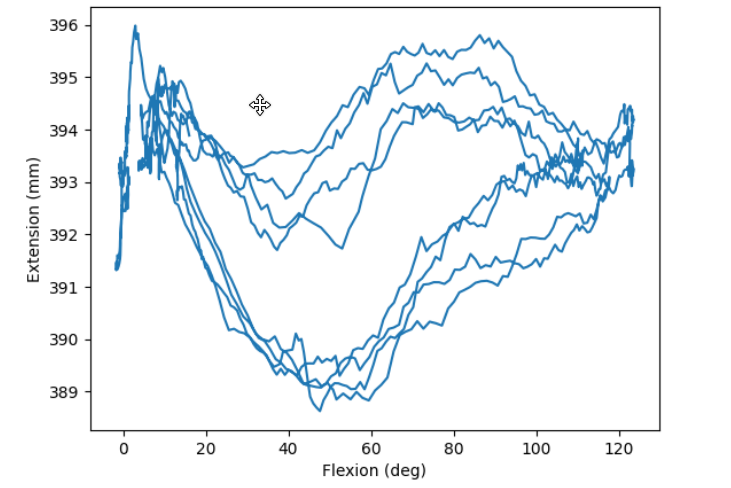
\includegraphics[width=\textwidth]{Figures/Param/Subj1_KneeProfile.png}
    \caption{A visualization of the angular flexion and linear extension of the shank from the joint center of the first dataset}
    \label{fig:Subj1KneeParams}
\end{figure}

\begin{figure}[ht!]
    \centering
    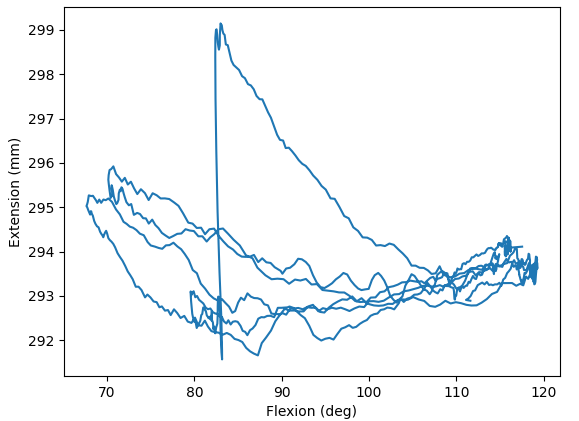
\includegraphics[width=\textwidth]{Figures/Param/Subj2_KneeProfile.png}
    \caption{A visualization of the angular flexion and linear extension of the shank from the joint center of the second dataset}
    \label{fig:Subj2KneeParams}
\end{figure}

The data displayed in \autoref{fig:Subj1KneeParams} has a variation of up to \(7mm\) for any given angle. However, what is most interesting is the difference in the direction of the flexion. When the knee joint angle is increasing (knee is being bent), the markers are closer together, compared to when the knee joint is decreasing. In any given direction of movement, variation is less than \(2mm\), suggesting that this seemingly cyclical trajectory is not due to measurement variations or inaccuracies.

\autoref{fig:Subj2KneeParams}'s data is seemingly less dependent on the knee joint angular velocity direction. All data is within a \(3mm\) variation at any given angle. The notable exception is the \(7mm\) spike that can be seen at roughly \(25^\circ\) mark. This can likely be explained by either an accidental shift in the markers or a slight measurement error in the motion capture system. However, there is not sufficient data to make a conclusion as to the reasoning.

The data analyzed both show that the maximum variation in skin movement through the flexion of the knee never exceeded \(7mm\), even with the outlier event from \autoref{fig:Subj2KneeParams}. In comparison, studies presented in \autoref{sec:KneeModel} describe a tibio\-femoral relationship that varies over \(40mm\) throughout the joint flexion. While these two data points are not statistically significant enough to make a conclusion for all human knees, the preliminary pilot data suggests that the skin movement is different than the tibiofemoral movement. An in-depth study is needed to make a definitive conclusion.

\section{Study Outline}

As a part of this thesis, an study was designed to test the developed parameterization software as well as the knee joint's capability to be customized to a specific person. However, due to time constraints, IRB (Internal Review Board) approval to run the human study was not obtained, and therefore the study was not run. The study's methodology is outlined below, and the IRB proposal documents are attached in \autoref{apx:ParamStudyDocs}.

Up to 6 subjects are to be selected to partake in this study. Each subject should not have any prior severe knee injury, and should be cleared to be imaged with an MRI. The study will start with imaging the knee using the motion capture procedures outlined in \autoref{sec:ImaginKneeProcedure}, and parameters will be selected using the parameterization software developed. These parameters will be used to manufacture an MRI safe personalized knee joint. Additionally, a second non-personalized pin joint will be manufactured and used as a control.

The second stage of the study will compare the fit of the two joints. The subject will undergo MR scans at up to 3 different knee angles, first with no joint and then subsequently with each type of joint. The movement (if any) of the joint in reference to the subjects body will be measured. A successful experiment should demonstrate that the customized knee joint moves less than a non-customized pin joint. Additionally, the tibiofemoral movement can be compared to the measured parameters to determine how much the skin moves relative to the knee joint.


    \chapter{Conclusion \& Future Work}

\section{Conclusion}

\begin{figure}[ht!]
    \centering
    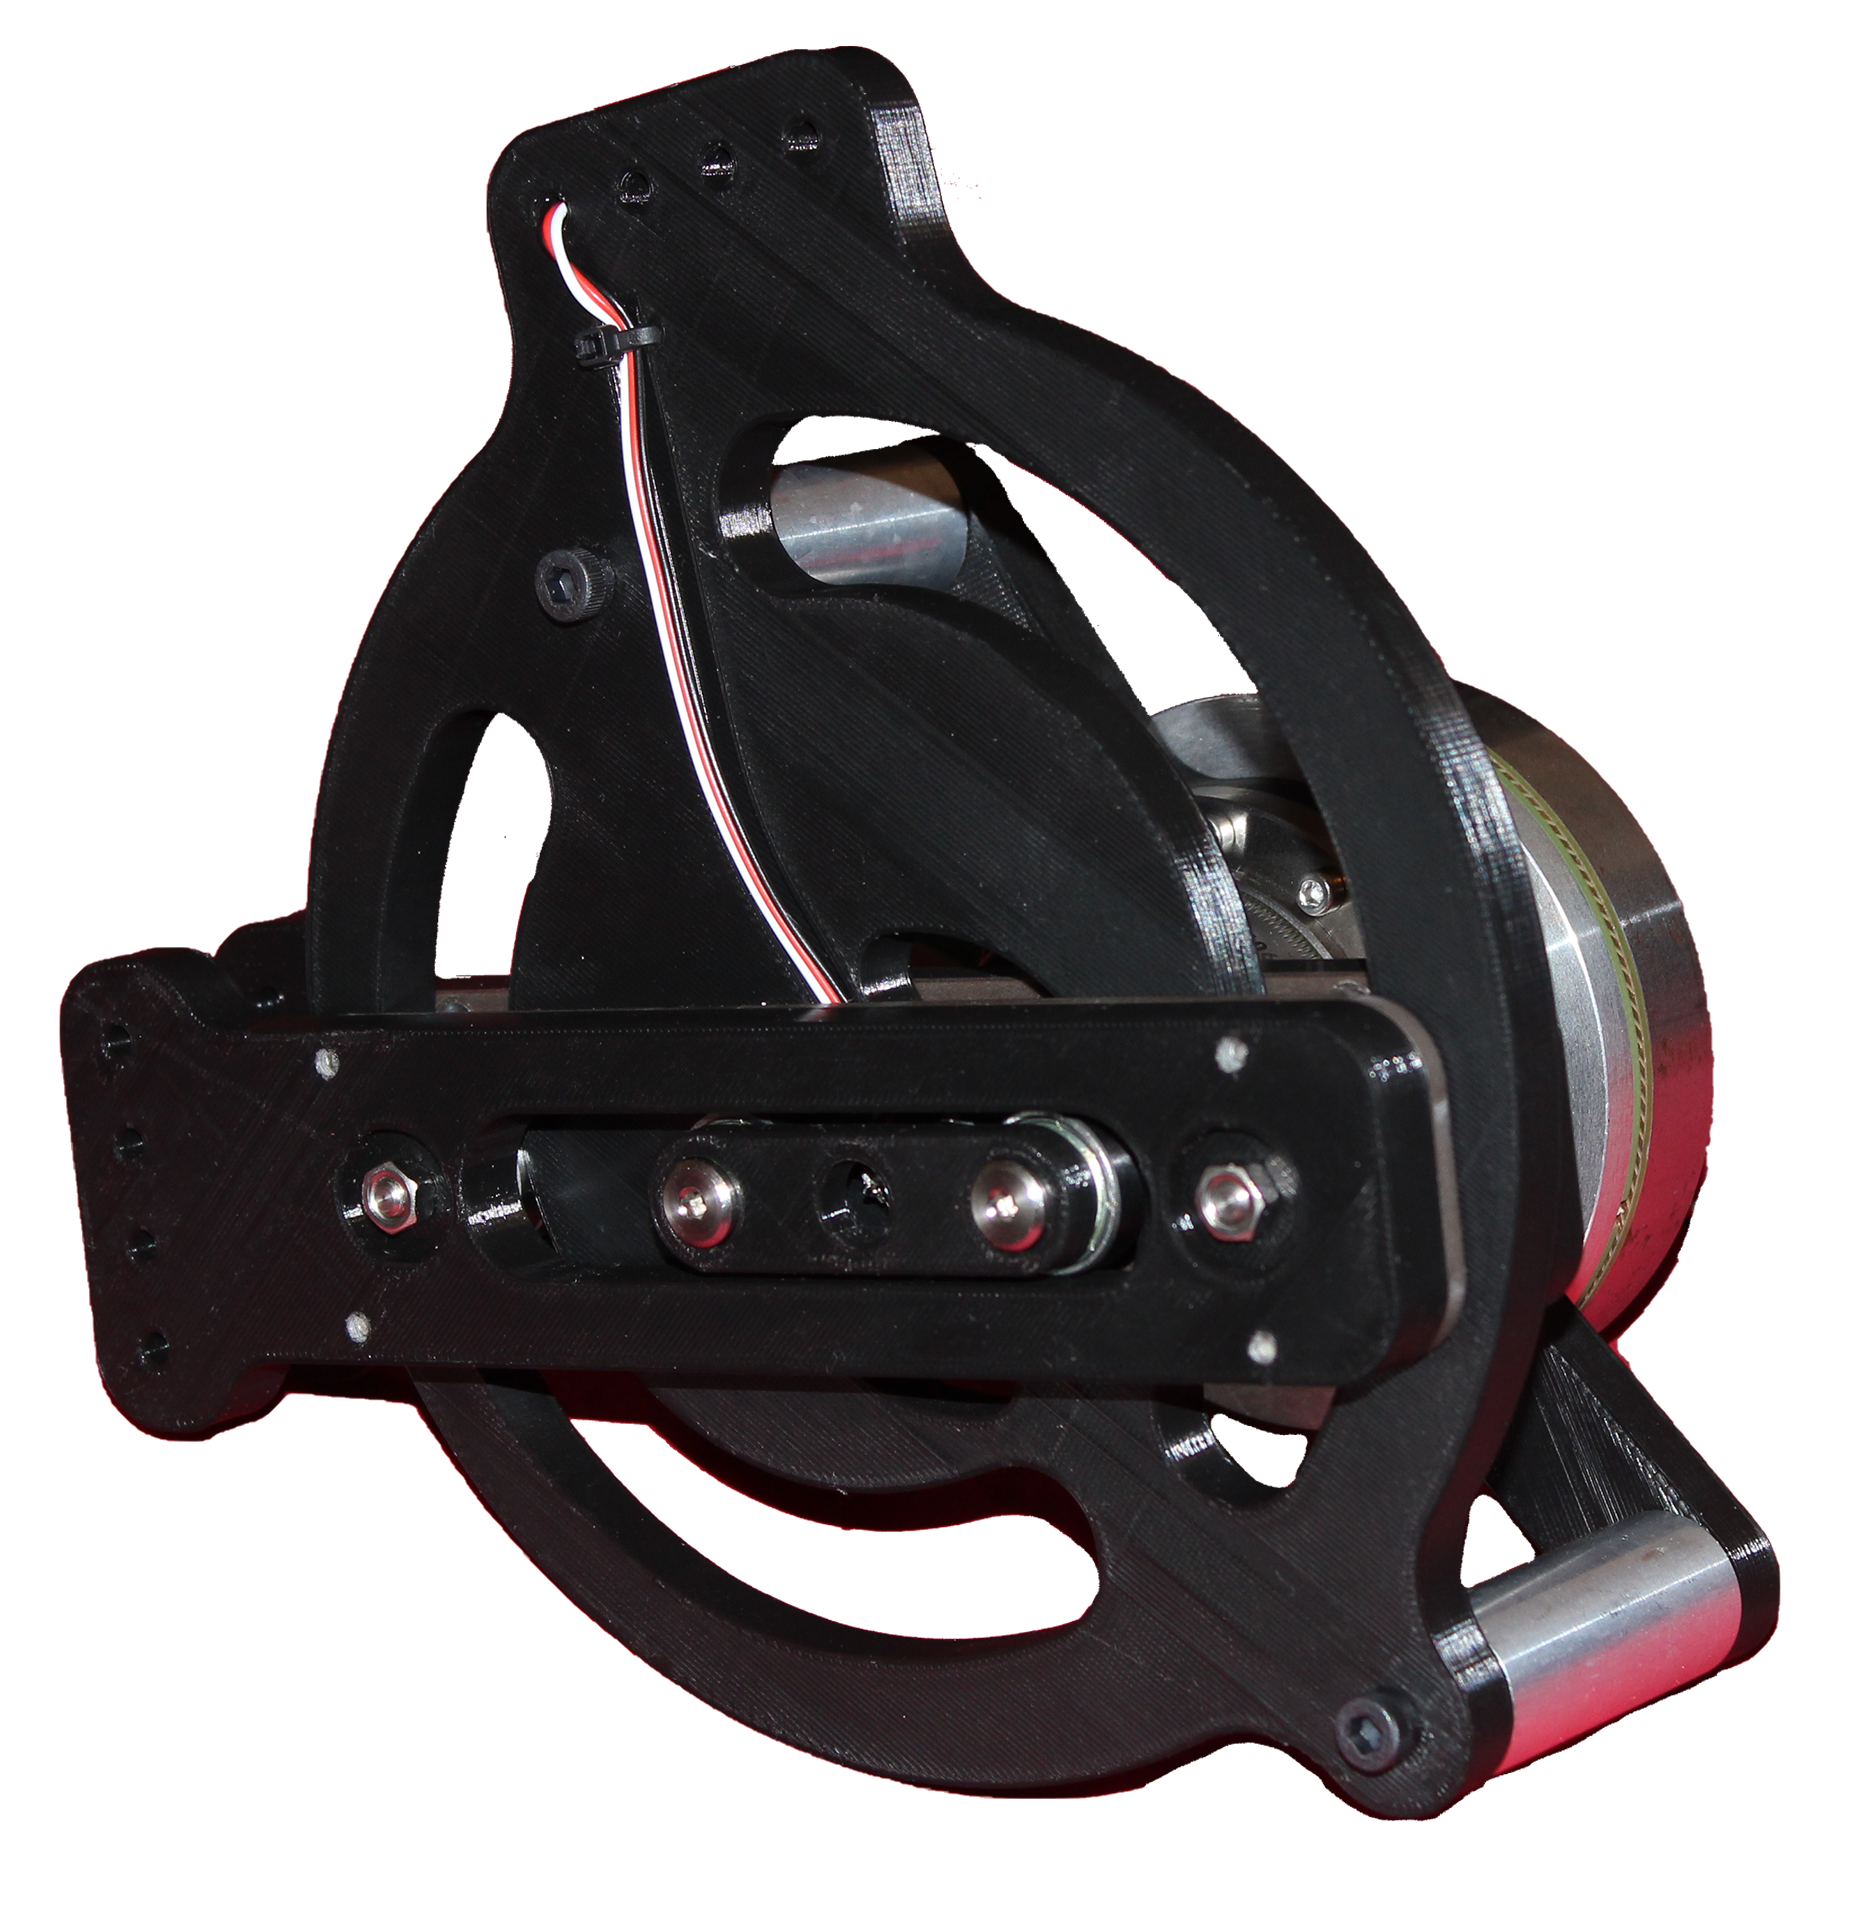
\includegraphics[width=0.7\linewidth]{Figures/KneeJointPrototype_ClearBackground.png}
    \caption{A picture of a left-sided knee joint prototype manufactured as a part of this thesis}
    \label{fig:KneeJointPicture}
\end{figure}

The proposed knee joint developed and tested in this thesis succeeded in all design requirements, even exceeding them in some scenarios. Experimentation showed that the knee could follow a defined tibiofemoral joint trajectory within \(1mm\) of accuracy. The joint itself can also be easily customized to each patient, with only one custom part needing to be manufactured per person per joint. Integrated sensors allow it to sense joint position and report it to the WPI LARRE hardware controllers. Strength analysis demonstrated that the joint can be manufactured from either PLA plastics using a conventional FDM 3D printer or machined out of aluminum. The joint will be able to support the stresses that come from common rehabilitation exercises including sit/stand exercises and walking gait exercises. Finally, the joint will be able to be integrated in the WPI LARRE (Legged Articulated Robotic Rehabilitation Exoskeleton). However, the design proposed is not limited to exoskeletons; the concept of using a cam mechanism to match tibiofemoral relationships can be applied to other orthoses that need to be powered.

\begin{figure}[ht!]
    \centering
    % \missingfigure[]{Picture of Knee Joint}
    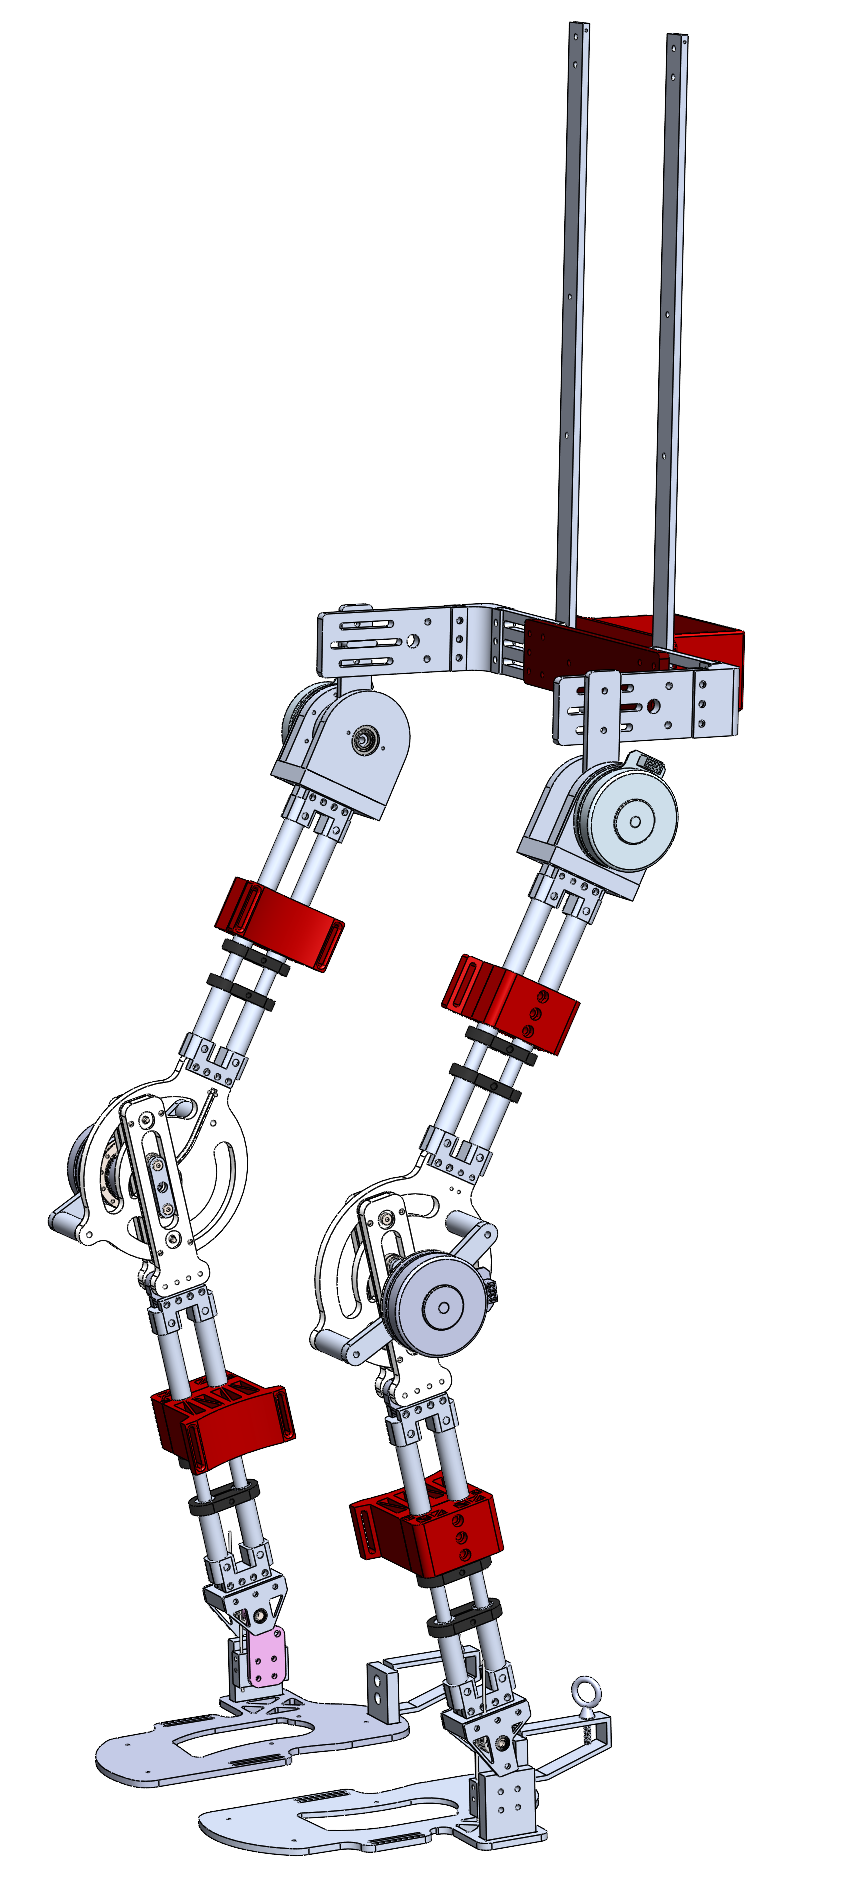
\includegraphics[width=0.4\linewidth]{Figures/FinalExoRender.png}
    \caption{Proposed knee joint mounted to a model of WPI LARRE}
    \label{fig:KneeOnExo}
\end{figure}

% TODO: Add conclusion for the knee parameterization

\section{Future Work}

While the design was able to match and even exceed the design requirements, more research is needed. From a design perspective, the joint can be made much smaller than the existing design. The motor and gearbox can be integrated in the joint to offer a lower profile exterior. Additionally, a more efficient and less expensive no-backlash gearbox such as a cycloidal gearbox can be integrated to replace the {Harmonic\texttrademark} gearbox used in this study. 

Additionally, more research is needed in knee movement in an exoskeleton. The research discussed in \autoref{sec:KneeModel} demonstrates the relationship between the tibia and femur, and does not look how skin movement changes the trajectory. Studies using the parameterization method discussed in \autoref{sec:KneeParams} may demonstrate a more accurate relationship to be used with this knee joint, as well as determine the parameters of a patient's knee. This would create a future where a lower-limb paralysis patient would be able to receive a perfectly personalized knee joint for their rehabilitation exoskeleton using an imaging system.
    
    % Print Bibliography
    \printbibliography[heading=bibintoc]

    \appendix

\chapter{Joint Power/Torque/Speed Calculations}
\label{apx:JointPowerTorqueSpeedCalcs}

\begin{equation}
    P_{output} = \epsilon P_{input} 
     \label{eq:PowerCalc}
\end{equation}

\begin{equation}
    \tau_{output} =   \frac{n_1}{n_2}  \epsilon  \tau_{input}
    \label{eq:TorqueCalc}
\end{equation}

\begin{equation}
    \omega_{output} = \omega_{input}  \frac{n_2}{n_1}
    \label{eq:SpeedCalc}
\end{equation}

\chapter{Maxon Motor EC90 Datasheet}
\label{apx:EC90Datasheet}
Below is the datasheet for the motor chosen for this project: Maxon EC90 part number 429271 (highlighted)
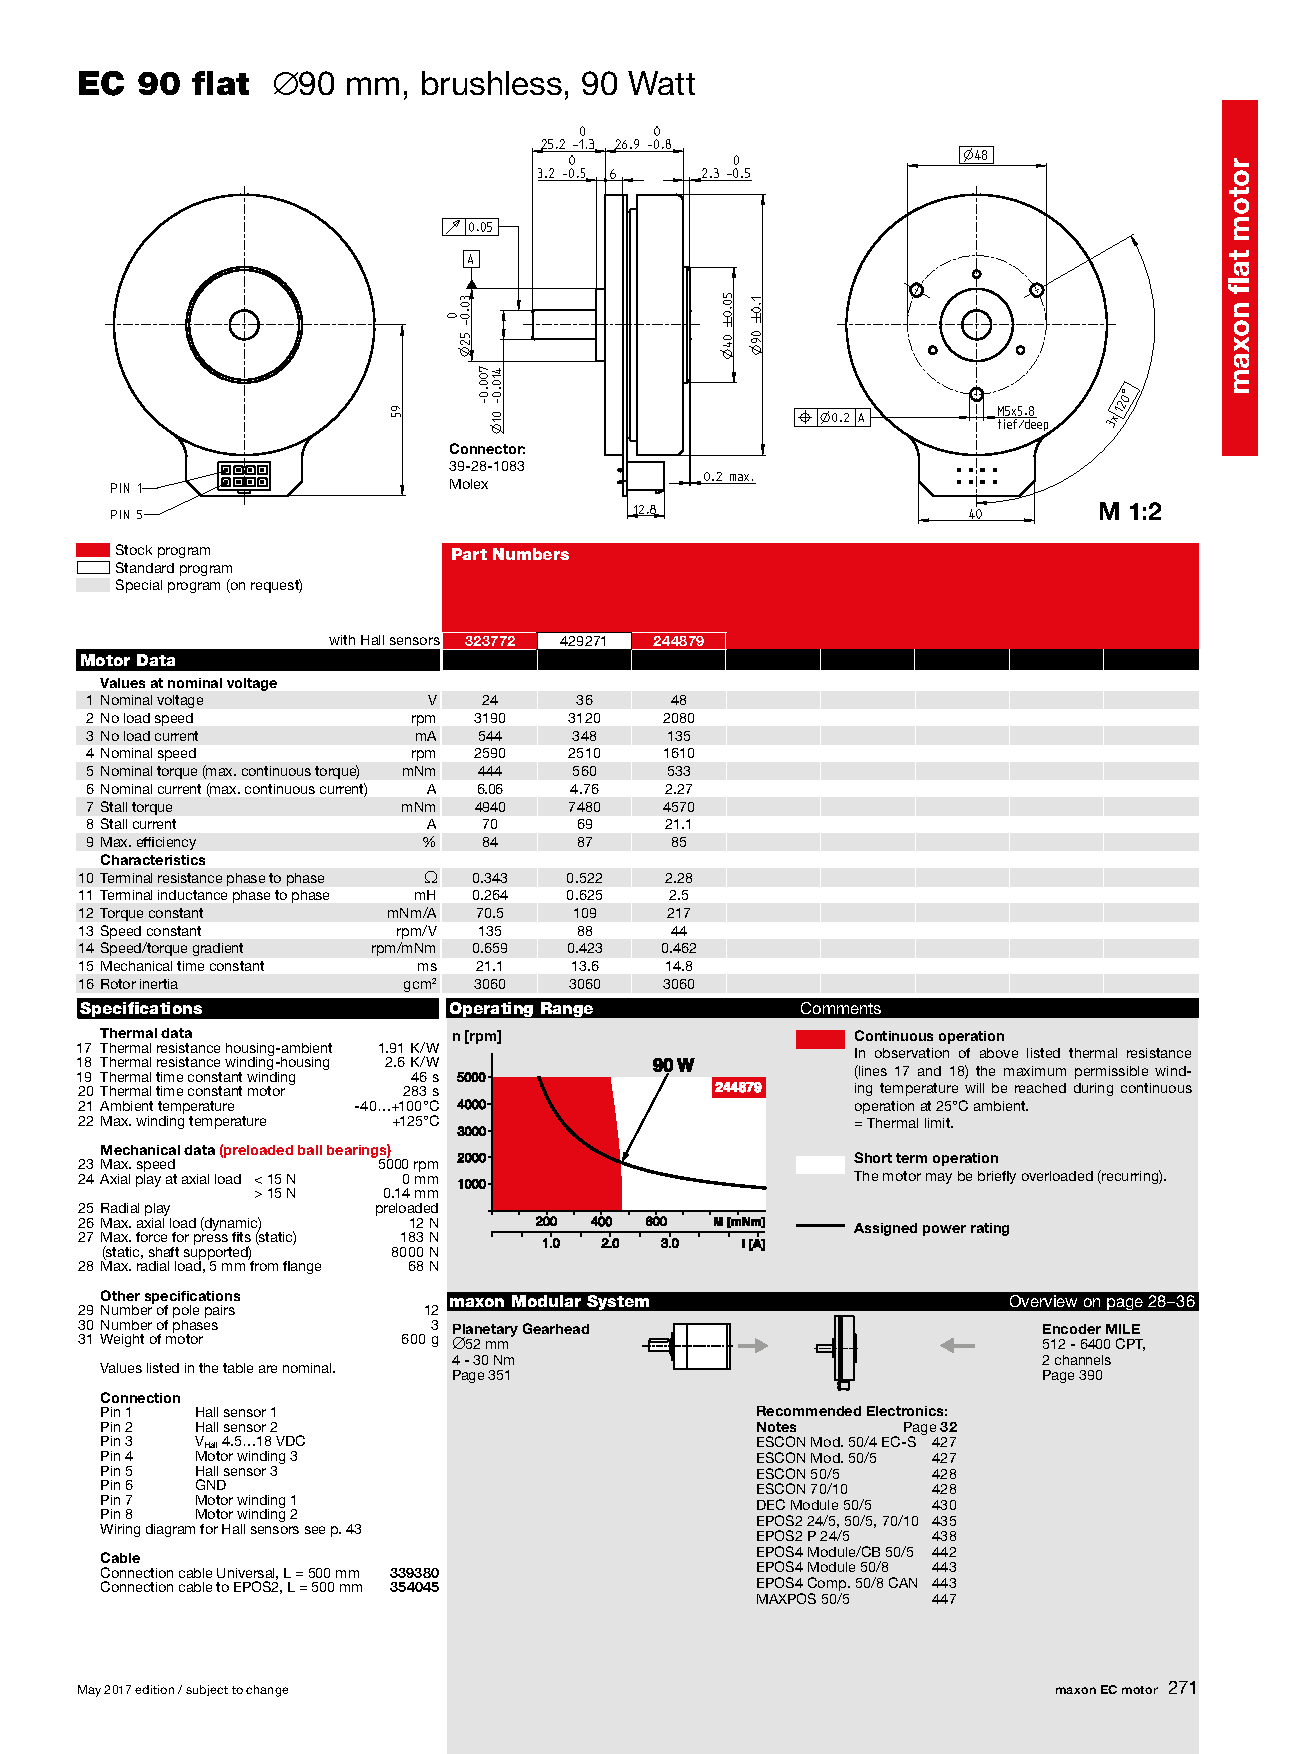
\includepdf[]{Appendix/EC90_Specs.pdf}



\end{document}